%Alle Gegenstände, die der iFSR zum Verleih anbietet

\documentclass[a4paper]{article}
\usepackage{german, graphicx}
\usepackage{ifthen}
\usepackage[utf8]{inputenc}
\usepackage{eurosym}
\usepackage{array}
\usepackage{booktabs}
\usepackage{grffile}

\newcommand{\iFS}{Fachschaft Informatik}
\newcommand{\iFSR}{FSR Informatik}

\newcommand{\infobox}[3] %Wie bekommt man den bloeden Text vertikal in die Mitte? pls fix me
        {\par
                \begin{tabular}{| c | c | c| }
                \hline
                Anzahl: #1 & Ausleihgebühr: \EUR{#2}   \\
                \hline
                \end{tabular} \\
        }                



\pagestyle{empty}

\begin{document}

\title{\bf Leihmaterialien des \iFSR \\
        der Technische Universität Dresden \\~\\
         
\includegraphics[width=.3\textwidth]{fsrlogo}
}

\maketitle

%Die hier aufgelisteten Materialien werden vom iFSR zum ausleihen angeboten.

\tableofcontents


\pagebreak

\section{Elektronische Geräte}

\subsection{Gigabit-Switch}
\infobox{1}{10}{Neu}
24-Port Gigabit Desktop/Rackmount Switch von TP-Link, Model Nummer TL-SG1024D. \\
\textbf{ Teile:} Switch, 2$\times$ Handbuch, schwarzes Kaltgerätekabel, Verpackung

%\subsection{Oculus Rift Dev Kit 2}
%\infobox{1}{30}{Neu}
%Das Oculus Rift ist ein Head-Mounted Display mit einem großen Sichtfeld und schnellen Bewegungssensoren. \\
%\textbf{Teile:} Headset mit Kabel, Stromadapter + 4 Aufsätze, Positionstracker + USB Kabel + Sync Kabel , 2$\times$ Paar Linsen, Putztuch, Adapter DVI zu HDMI, Handbuch, Box

\subsection{Raspberry Pi B}
\infobox{2}{3}{Neu}
Ein Raspberry Pi ist ein Miniatur-Computer, der nicht viel größer als eine EC-Karte ist. Das Zubehör erlaubt es den Raspberry einfach an ein Netzwerk anzuschließen. \\
\textbf{Teile:}Raspberry Pi B(mit Kühlkörper), Gehäuse(schwarz), Netzteil micro-USB 2A , Wlan Adapter, HDMI-Kabel, 8 GB SD HC Samsung, Ethernetkabel (2m weiß), GPIO Breakout T-Cobbler, USB-TTL-Kabel 

 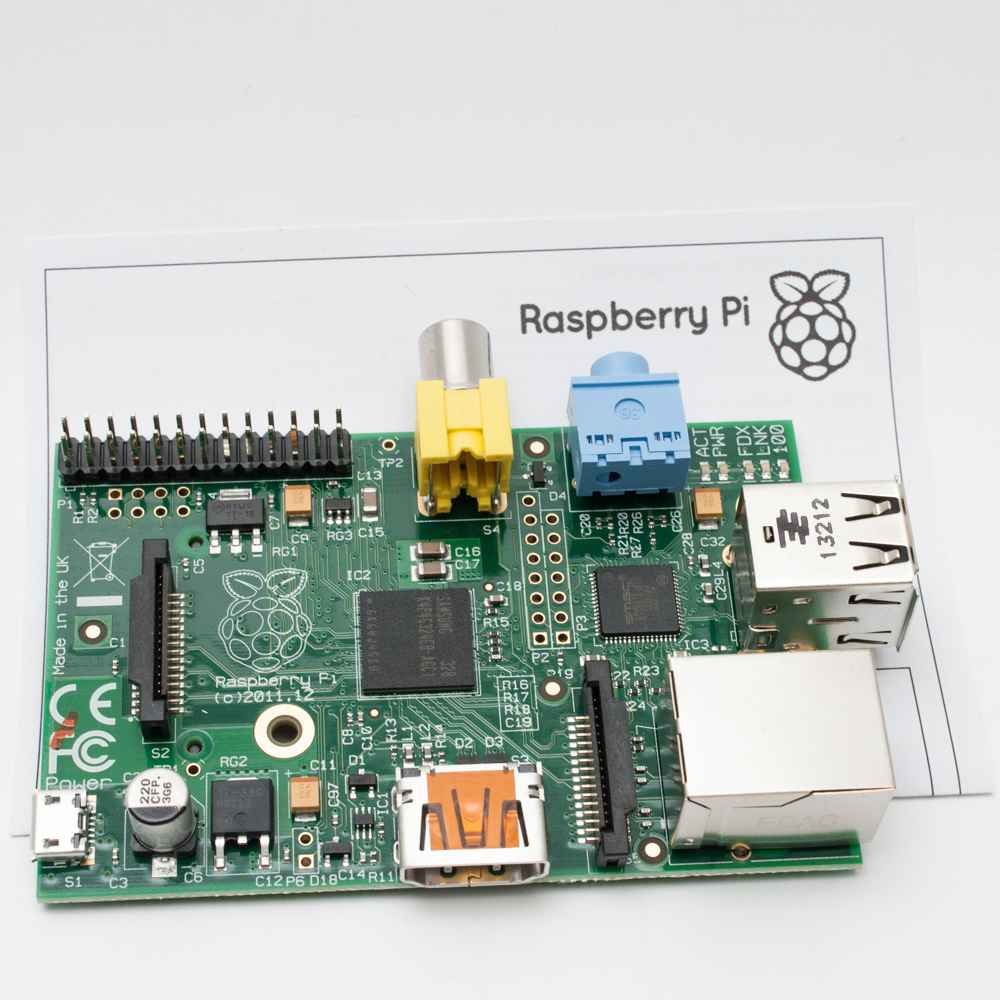
\includegraphics[width=.3\textwidth]{Raspberry Pi B.jpg}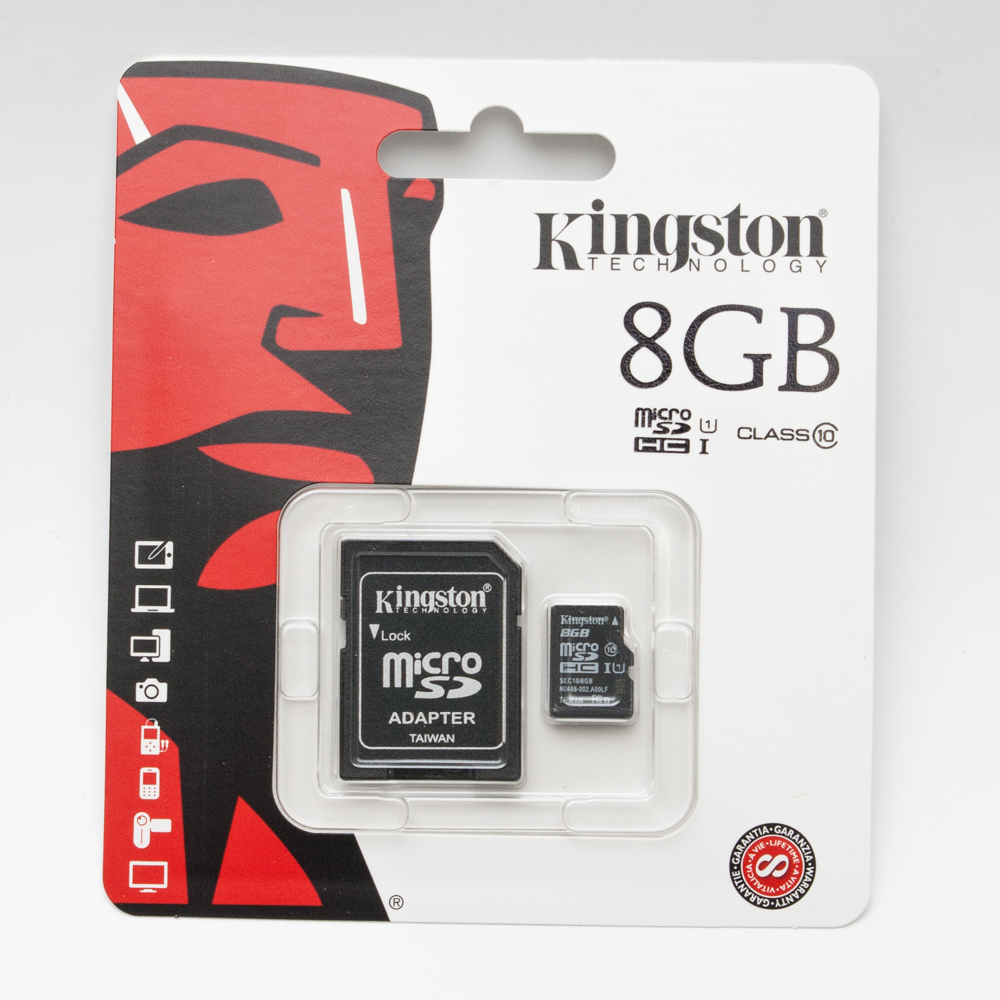
\includegraphics[width=.3\textwidth]{MicroSD 8GB Class 10.jpg} 
\includegraphics[width=.3\textwidth]{raspberryPiQR}

\subsection{Raspberry Pi B+}
\infobox{3}{3}{Neu}
Ein Raspberry Pi ist ein Miniatur-Computer, der nicht viel größer als eine EC-Karte ist. Das Modell B+ ist eine verbesserte Variante vom Modell B, unteranderem verbaucht er weniger Strom und hat mehr USB-Anschlüsse. \\
\textbf{Teile:} Raspberry Pi B+ (mit Gehäuse), Micro SD, aktiver USB-HUB, Micro-USB Kabel, GPIO Breakout T-Cobbler, USB-TTL-Kabel

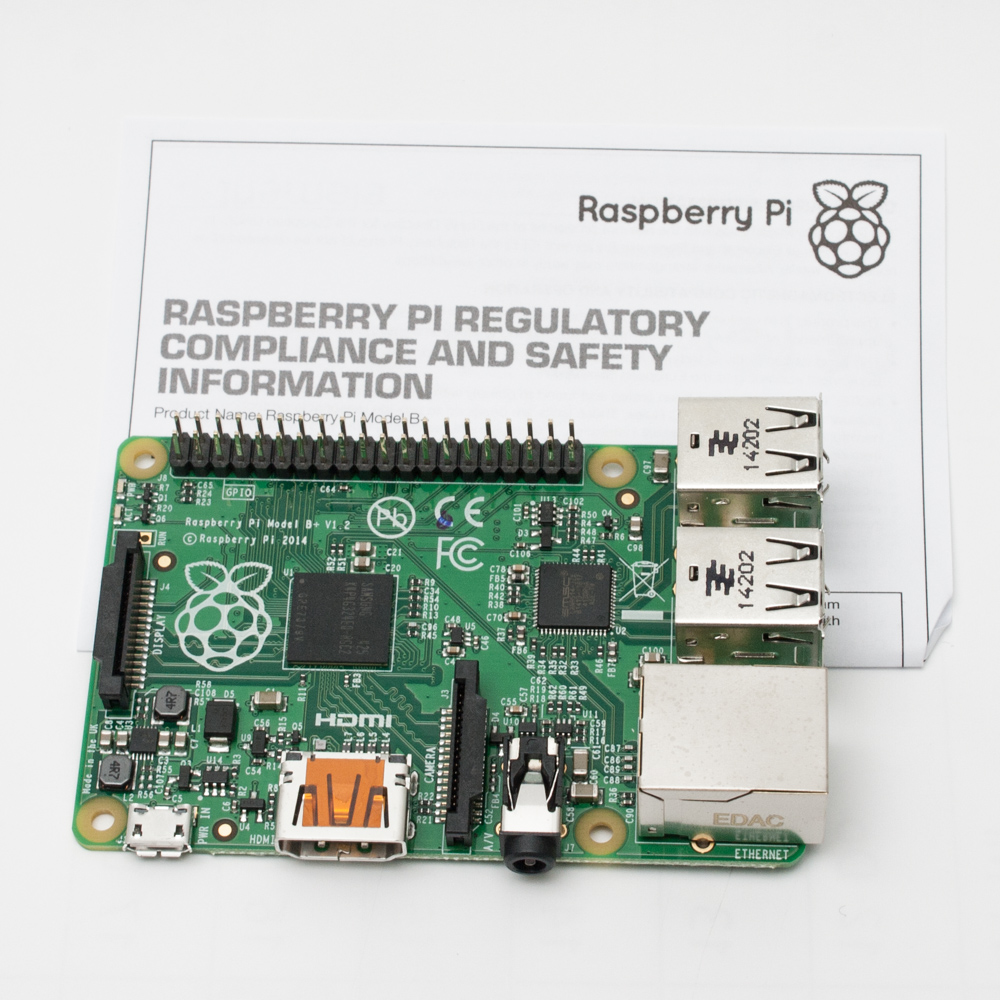
\includegraphics[width=.3\textwidth]{Raspberry Pi Bplus.jpg}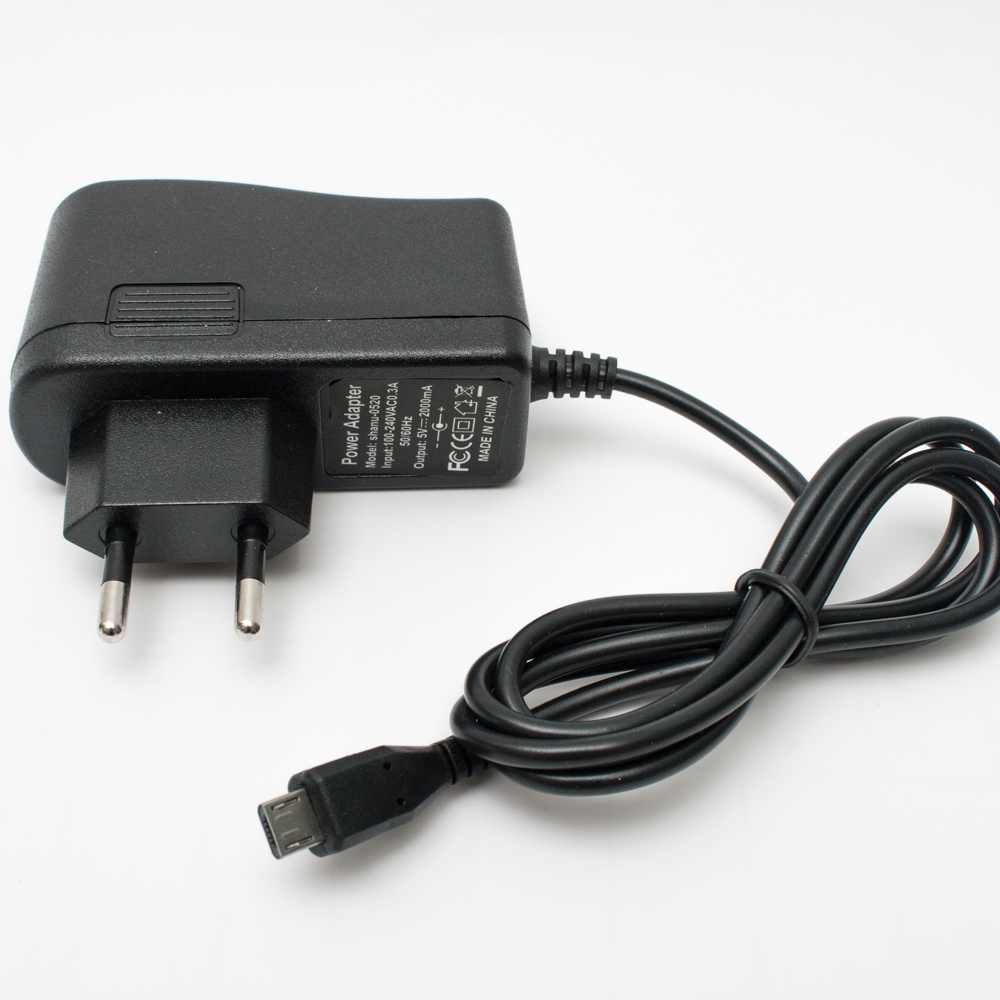
\includegraphics[width=.3\textwidth]{Netzteil USB 2A schwarz.jpg}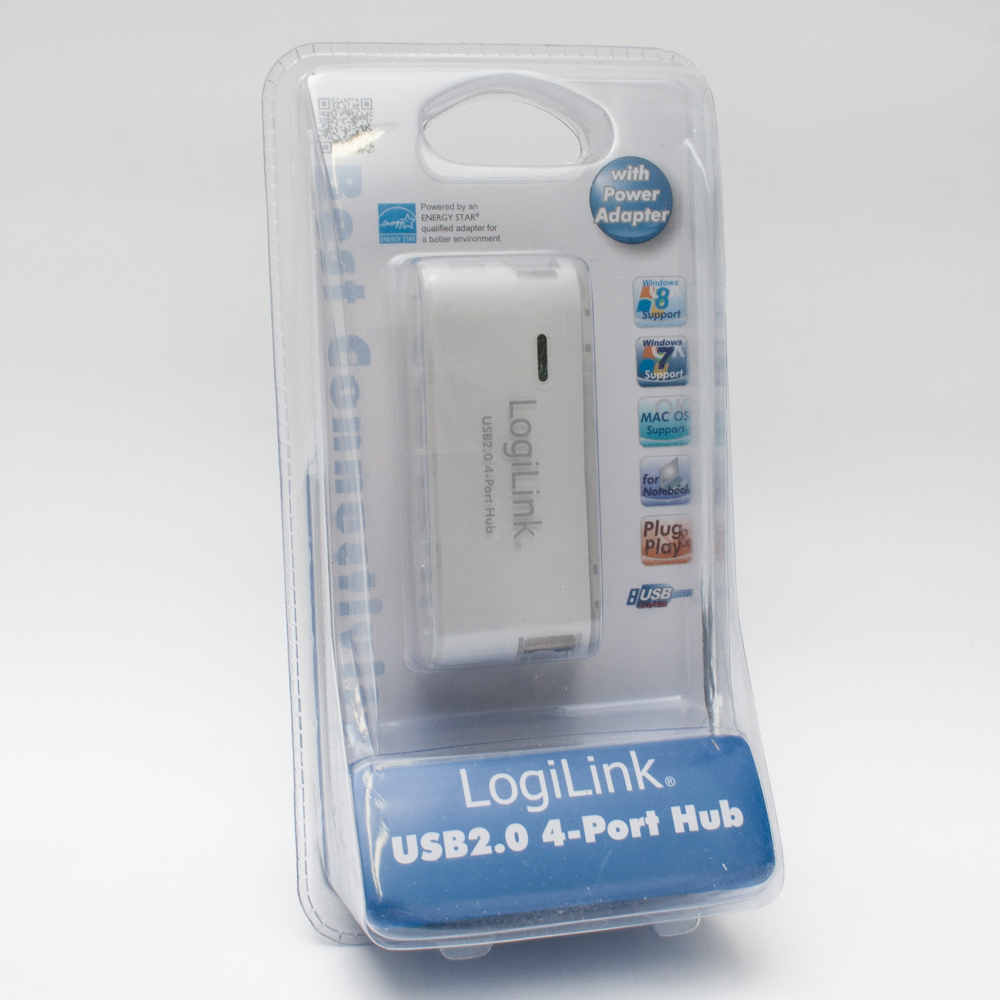
\includegraphics[width=.3\textwidth]{Aktiver USB-Hub.jpg}


\subsection{PiFace Rack}
\infobox{2}{2,5}{Neu}
Das PiFace Rack erlaubt das anschließen von bis zu 4 weiteren Platinen mit einem Raspberry Pi.\\
\textbf{Teile:}PiFace Rack

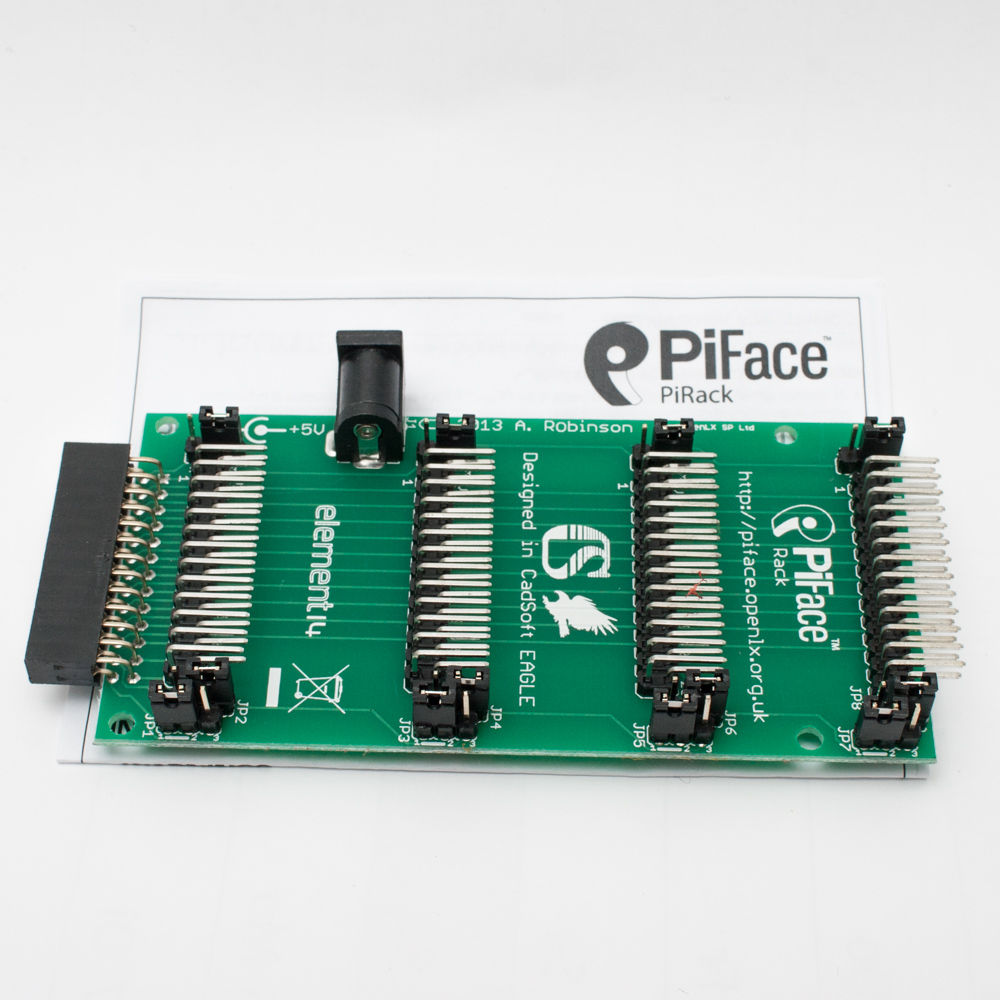
\includegraphics[width=.3\textwidth]{PiFace Rack.jpg}
\includegraphics[width=.3\textwidth]{PiFaceRack}

\subsection{PiFace Board}
\infobox{2}{2,5}{Neu}
Das PiFace Board ermöglicht es, über die Schraubverbindungen, angeschlossene Geräte mit einem Raspberry Pi zu verbinden.\\
\textbf{Teile:}PiFace Board

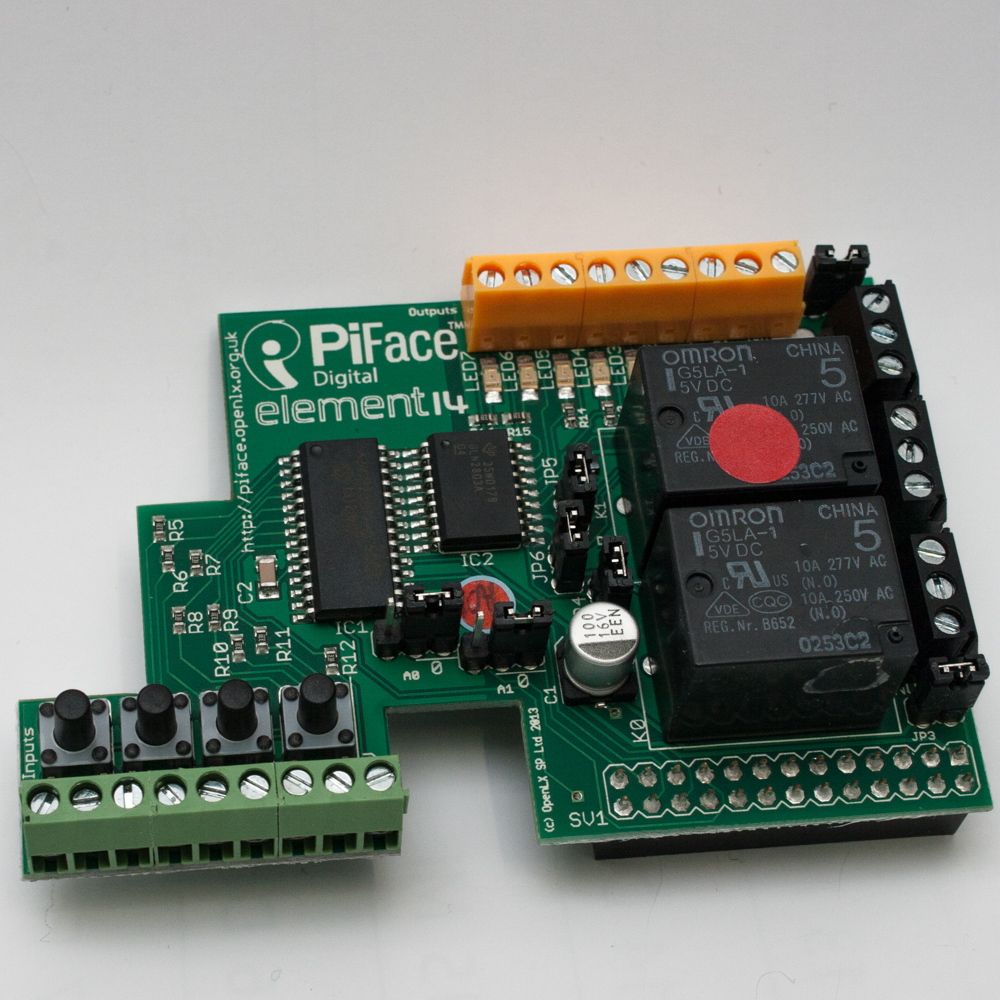
\includegraphics[width=.3\textwidth]{PiFace Board.jpg}

\subsection{Gertboard}
\infobox{2}{2,5}{Neu}
Das Gertboard ist eine Erweiterung für einen Raspberry Pi mit dem sich kleine elektronische Projekte realisieren lassen.\\
\textbf{Teile:} Gertboard

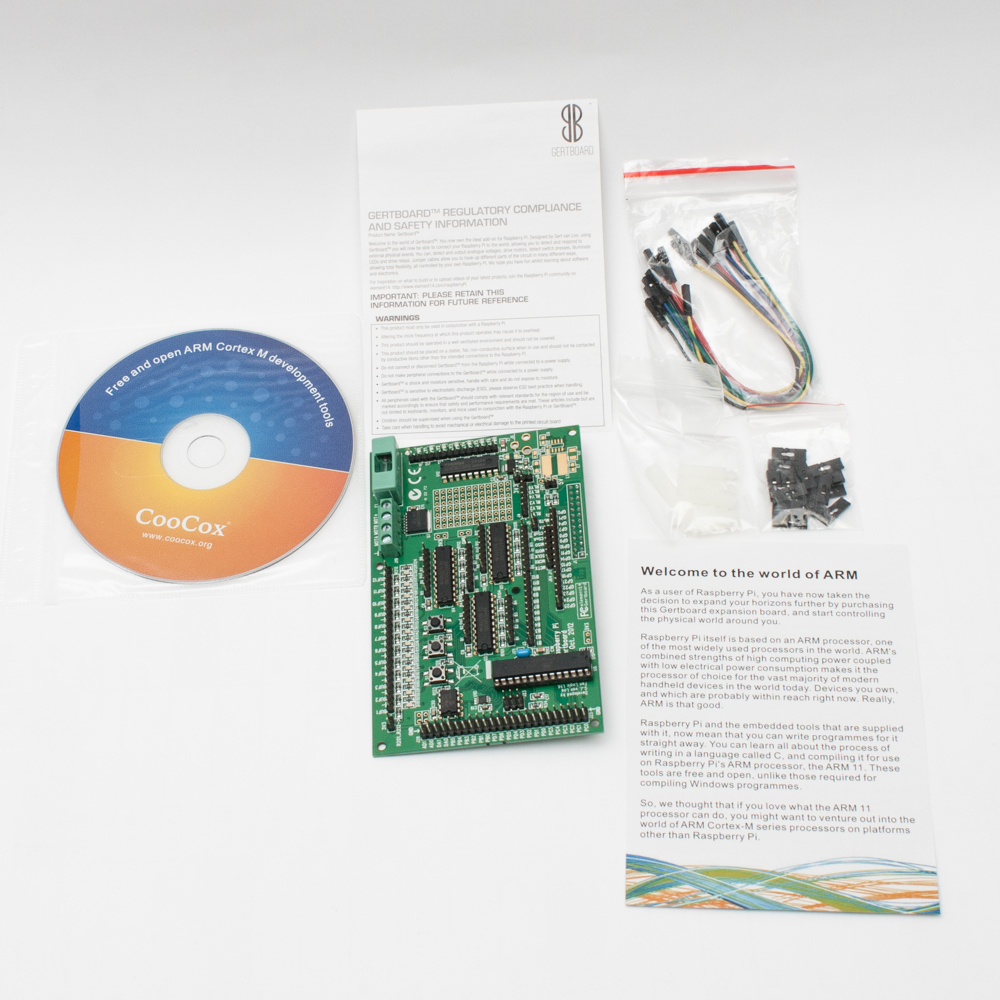
\includegraphics[width=.3\textwidth]{Gertboard.jpg}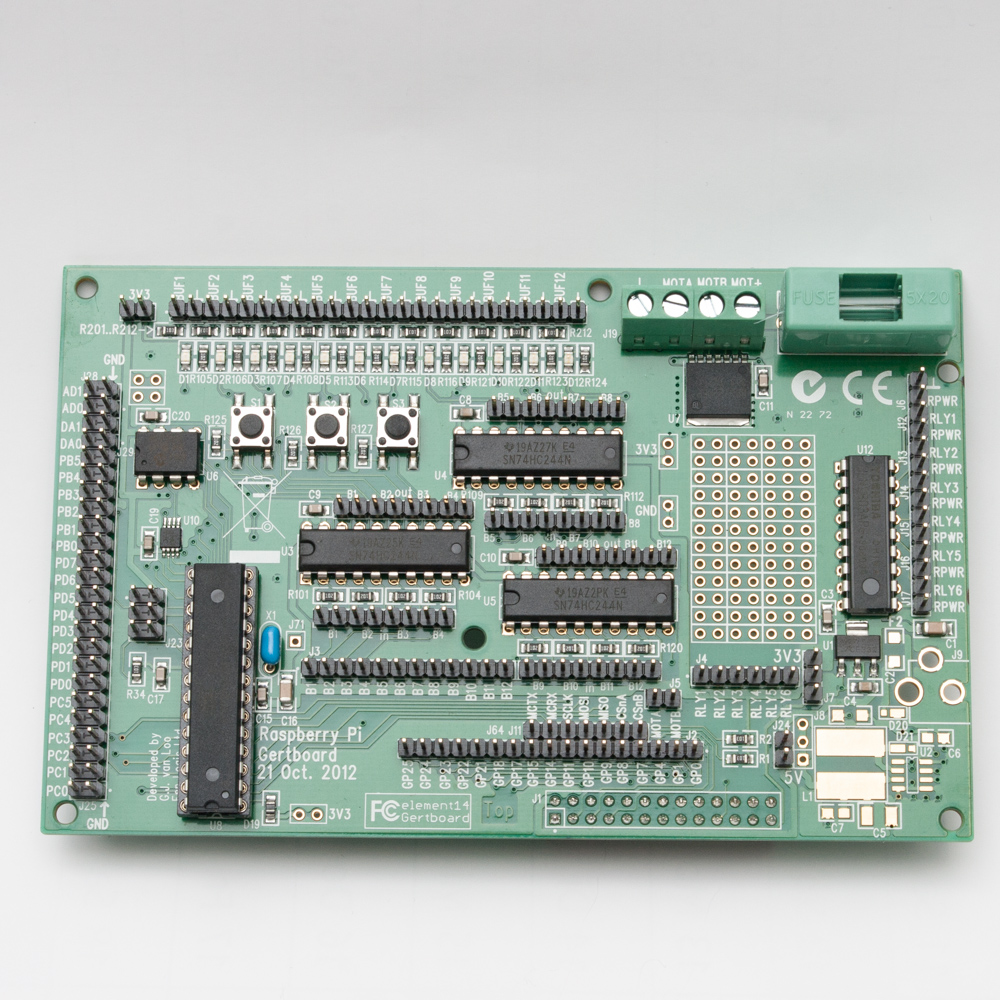
\includegraphics[width=.3\textwidth]{Gertboard-2.jpg}

\subsection{Embedded Pi Board}
\infobox{1}{2,5}{Neu}
Das Embedded Pi Board fungiert als Adapter zwischen einem Raspberry Pi und einem Adruino kompatiblen Schild. \\
\textbf{Teile:} Embedded Pi Board

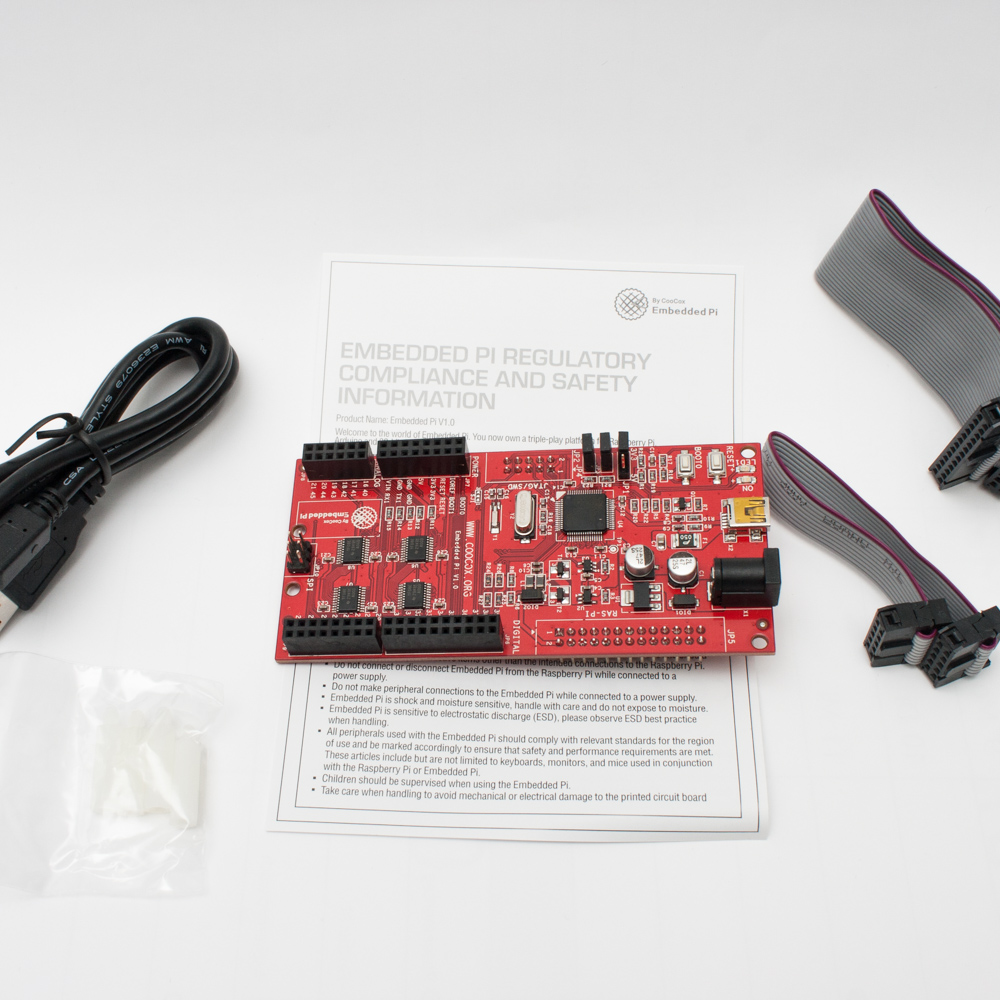
\includegraphics[width=.3\textwidth]{Embedded Pi Board.jpg}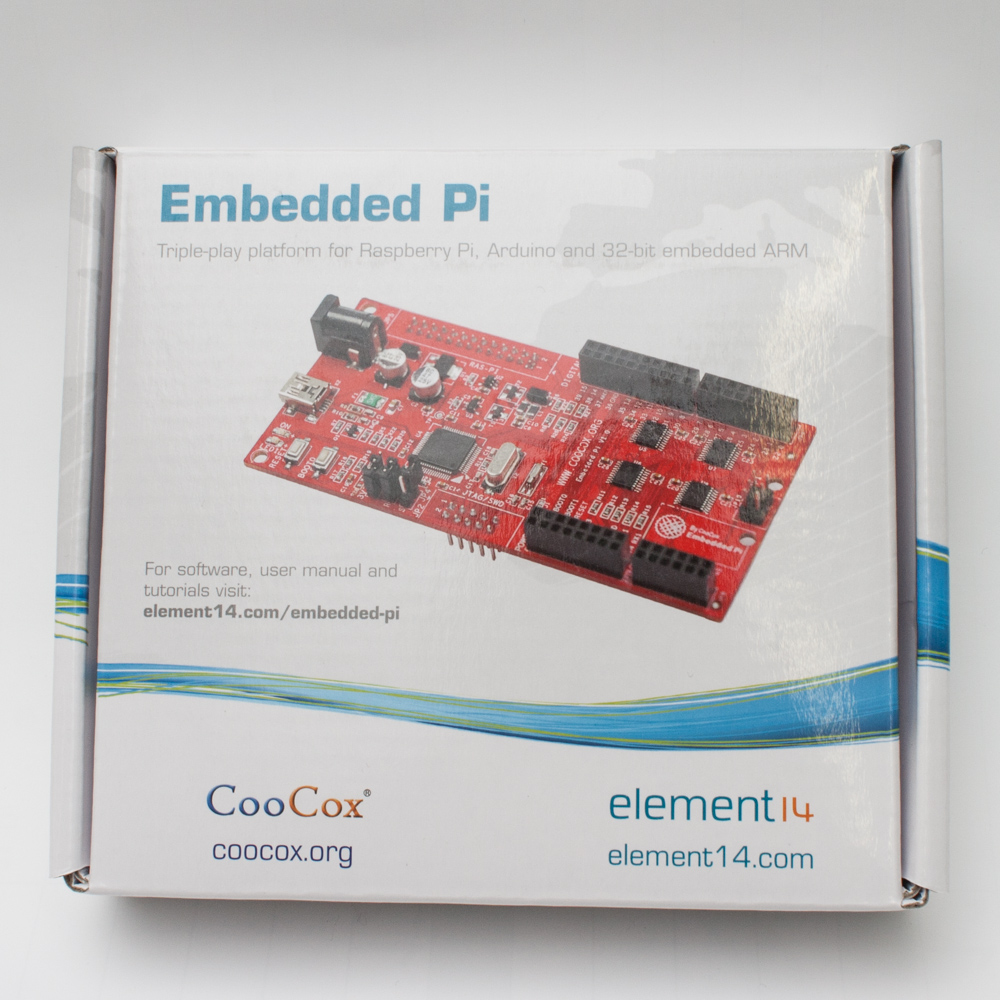
\includegraphics[width=.3\textwidth]{Embedded Pi Board-3.jpg}

\subsection{Pi Camera}
\infobox{2}{0}{Neu}
Ein Kamera-Modul für den Raspberry Pi.\\
\textbf{Teile:} Pi Camera, Halterung

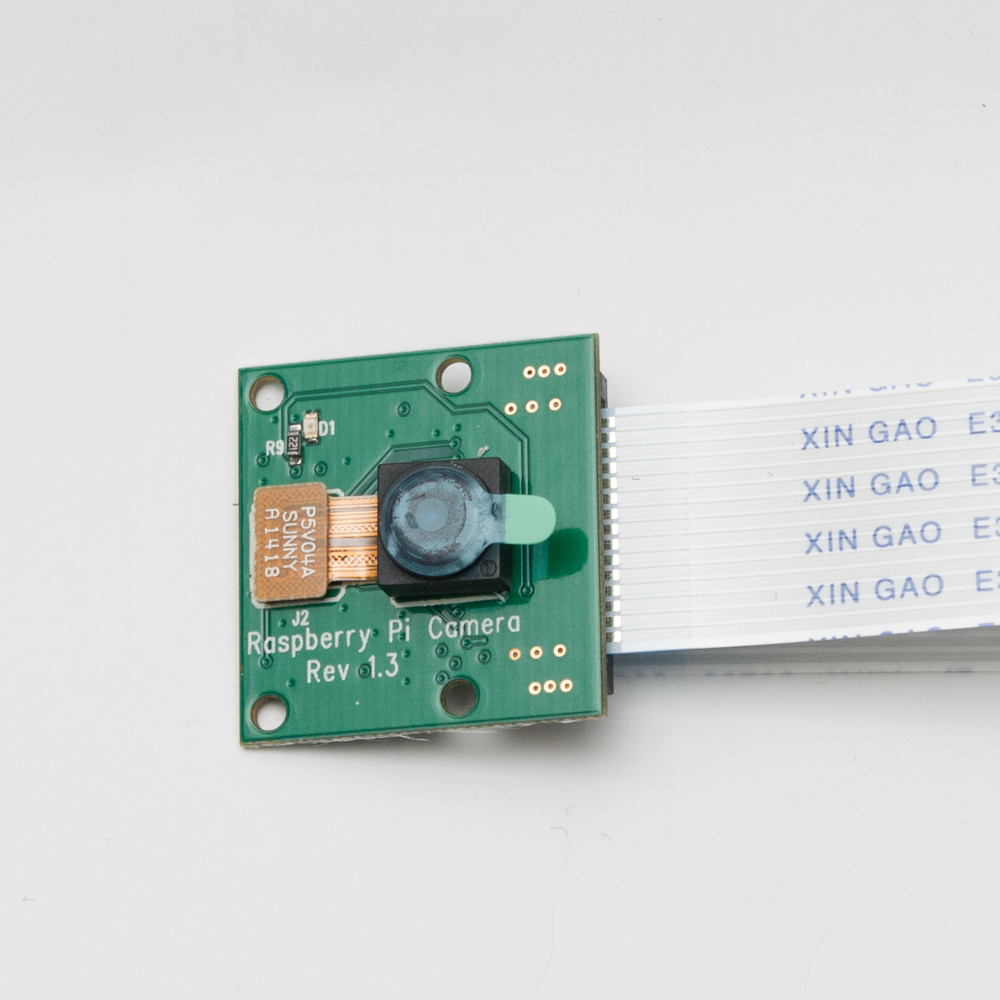
\includegraphics[width=.3\textwidth]{PiCam.jpg}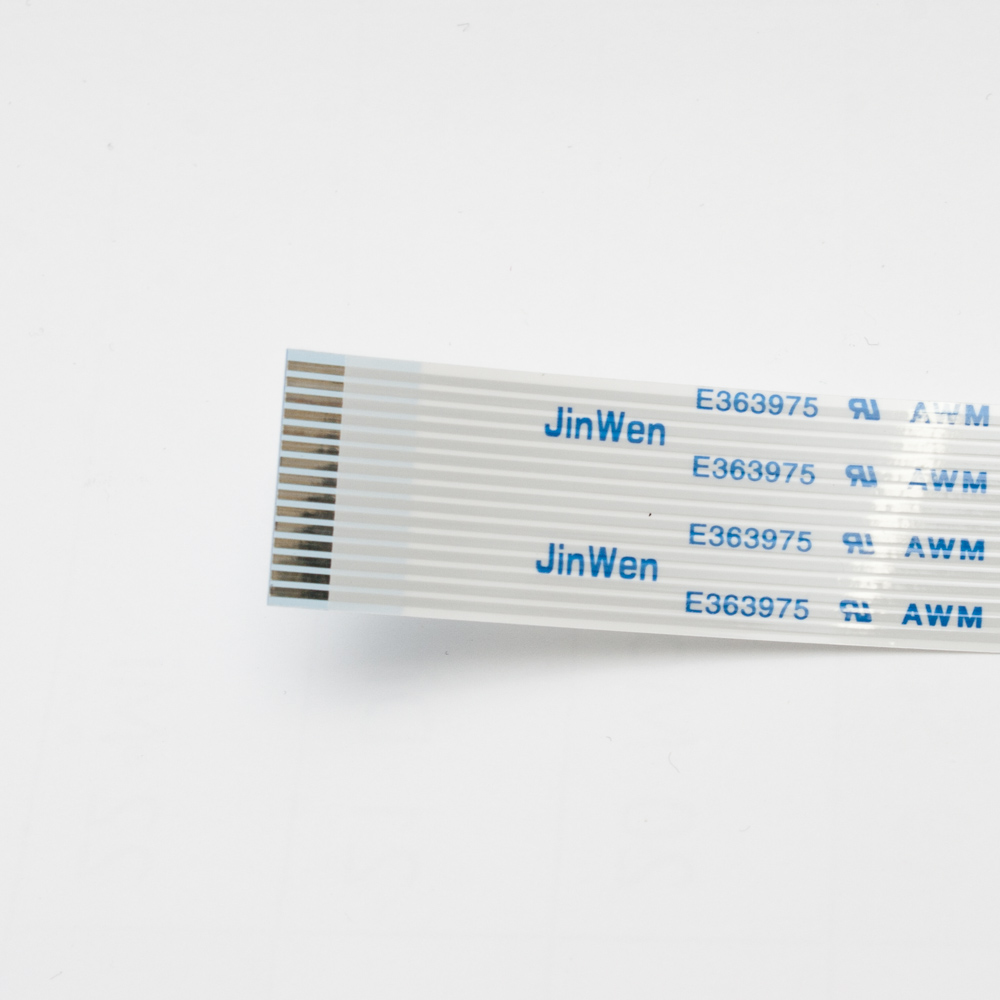
\includegraphics[width=.3\textwidth]{PiCam-Kabel.jpg}

\subsection{Pi Camera (Infrarot)}
\infobox{2}{0}{Neu}
Ein Kamera-Modul für den Raspberry Pi, kann auch Infrarot Bilder machen. \\
\textbf{Teile:} Pi Camera, Halterung, Kabelverlängerung, blauer Filter

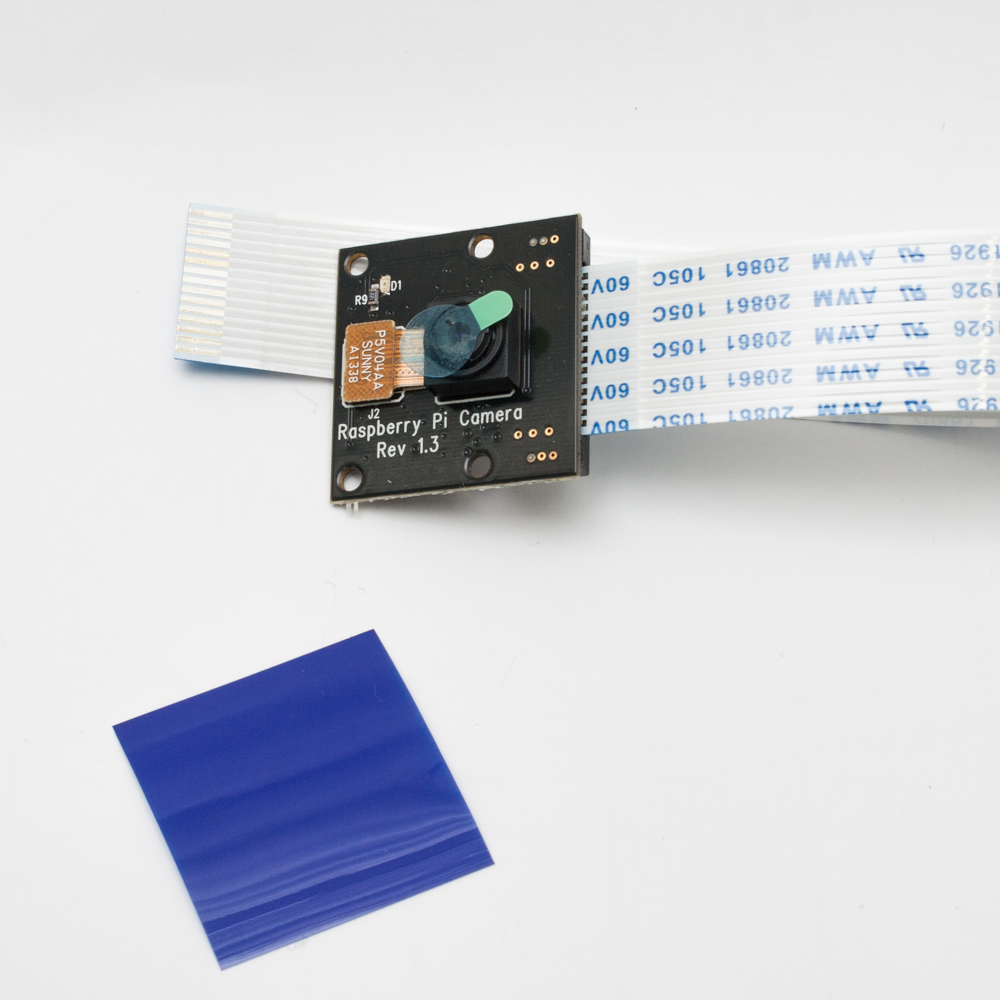
\includegraphics[width=.3\textwidth]{PiCam NoIR.jpg}

\subsection{Banana Pi}
\infobox{1}{0}{Neu}
Der Banana Pi ist ein Nachbau des Raspberry Pi mit besserer Hardware. \\
\textbf{Teile:} Banana Pi, Gehäuse, Netzteil 2A, HDMI-Kabel, Wlan-Dongel

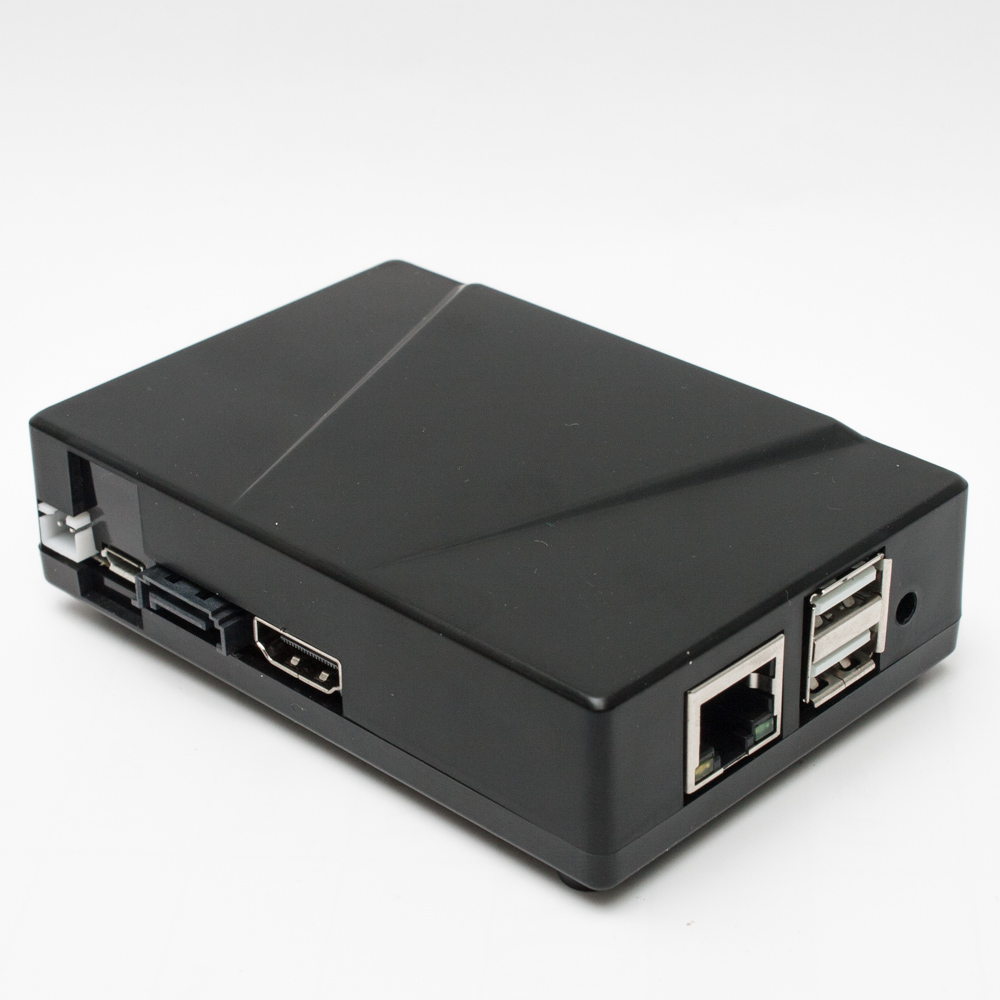
\includegraphics[width=.3\textwidth]{BananaPi.jpg}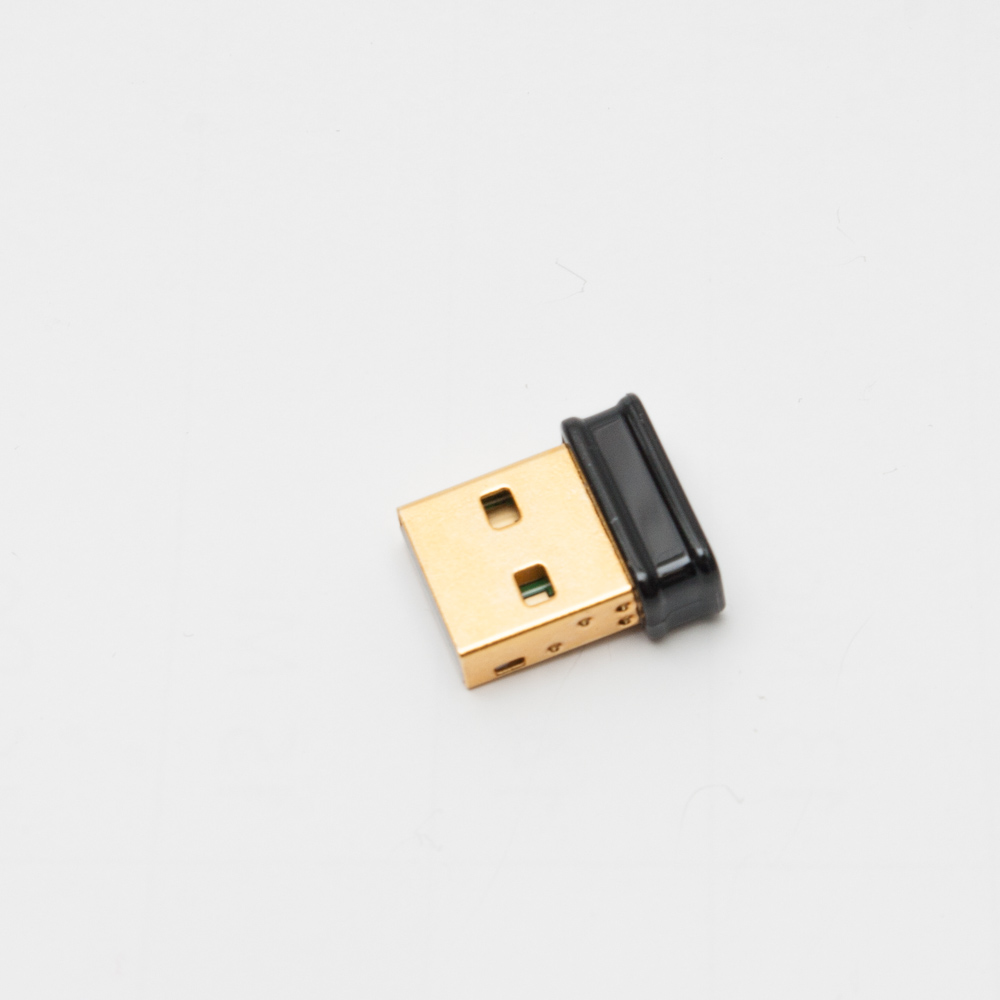
\includegraphics[width=.3\textwidth]{WLAN-Dongle.jpg}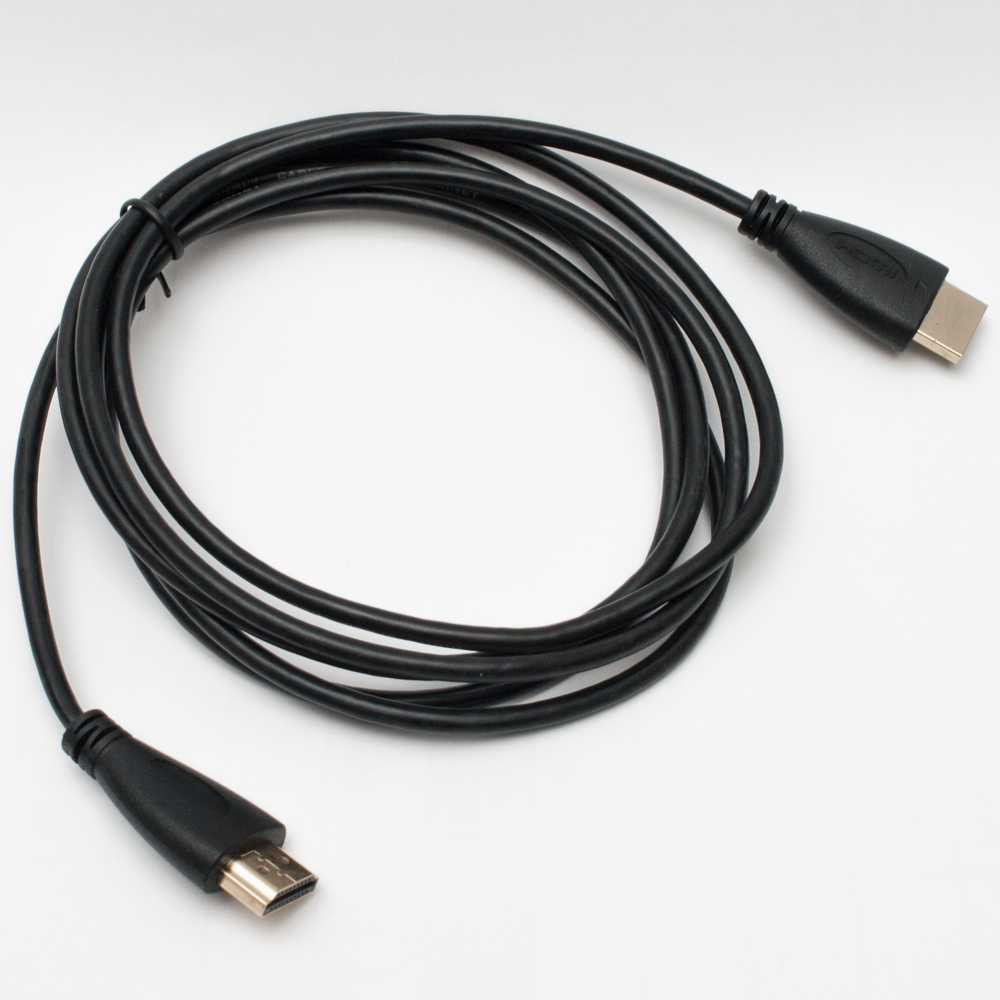
\includegraphics[width=.3\textwidth]{HDMI-Kabel schwarz.jpg}

\subsection{Adapter HDMI auf VGA}
\infobox{1}{0}{Neu}
Ein Adapter von einem HDMI Eingang auf einen VGA Ausgang. \\
\textbf{Teile:} Adapter HDMI auf VGA

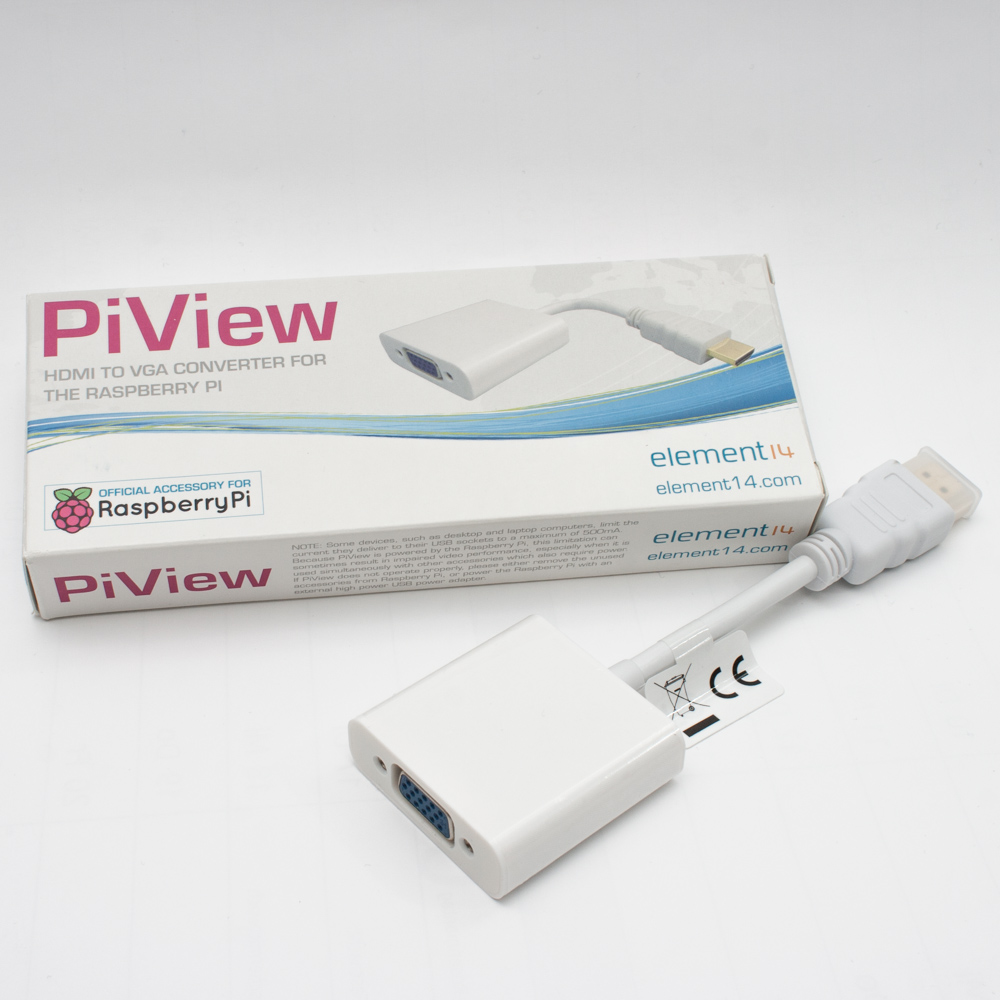
\includegraphics[width=.3\textwidth]{HDMI-VGA-Adapter.jpg}

\subsection{Cubietruck}
\infobox{1}{0}{Neu}
Ein Miniatur-Computer vom Cubieteam, hat unteranderem Wifi, VGA und Bluethooth onboard. \\
\textbf{Teile:} Cubietruck, Gehäuse, Kabel Mini-USB-Stecker/USB-A-Stecker, USB-Stromversorungskabel, Zusatz-Kühlkörper, Montagematerial

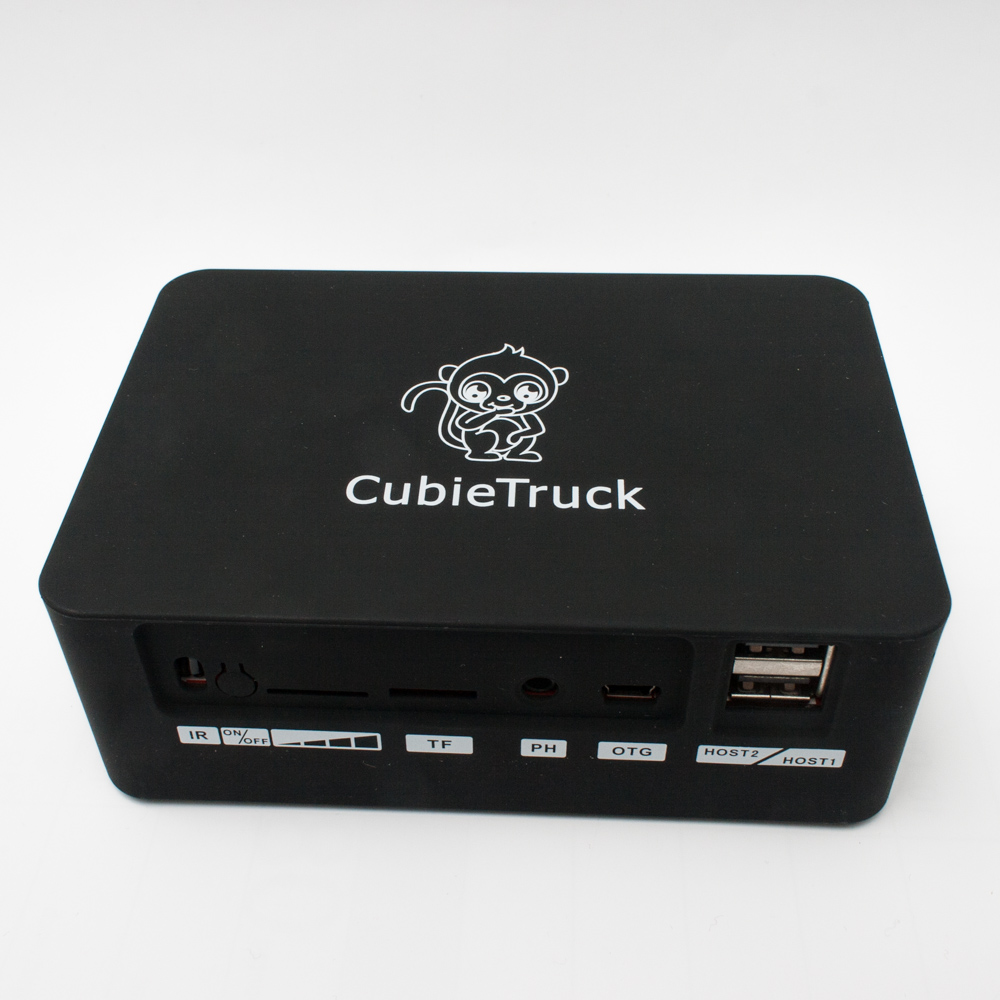
\includegraphics[width=.3\textwidth]{CubieTruck.jpg}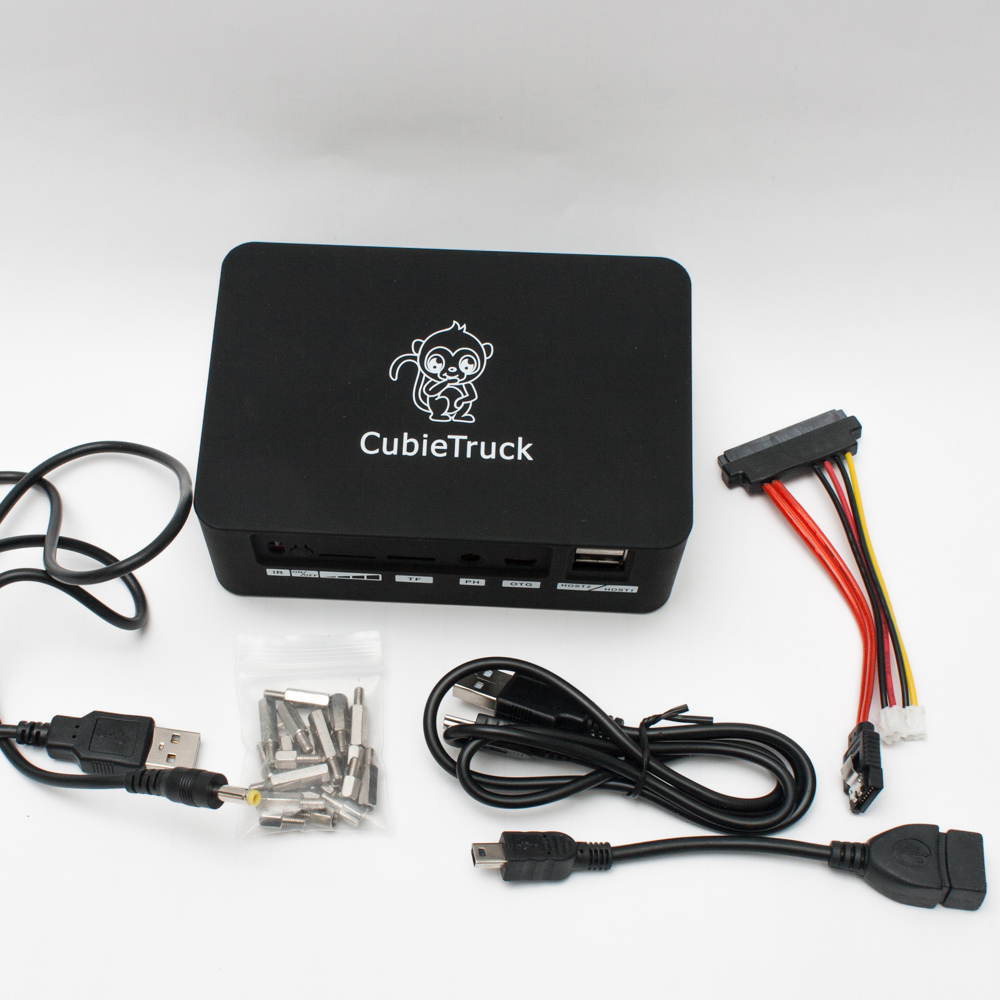
\includegraphics[width=.3\textwidth]{CubieTruck-2.jpg}

\subsection{Funduino-Lernset 6} 
\infobox{1}{2,5}{Neu}
Nachbau eines Arduinos mit vielen Teilen zum basteln und ausprobieren.\\
\textbf{Teile:} Funduino MEGA 2560 R3, Sensoren, Bauteile (details siehe QR-Code)
% http://funduino.de/index.php/shop/product/view/1/10

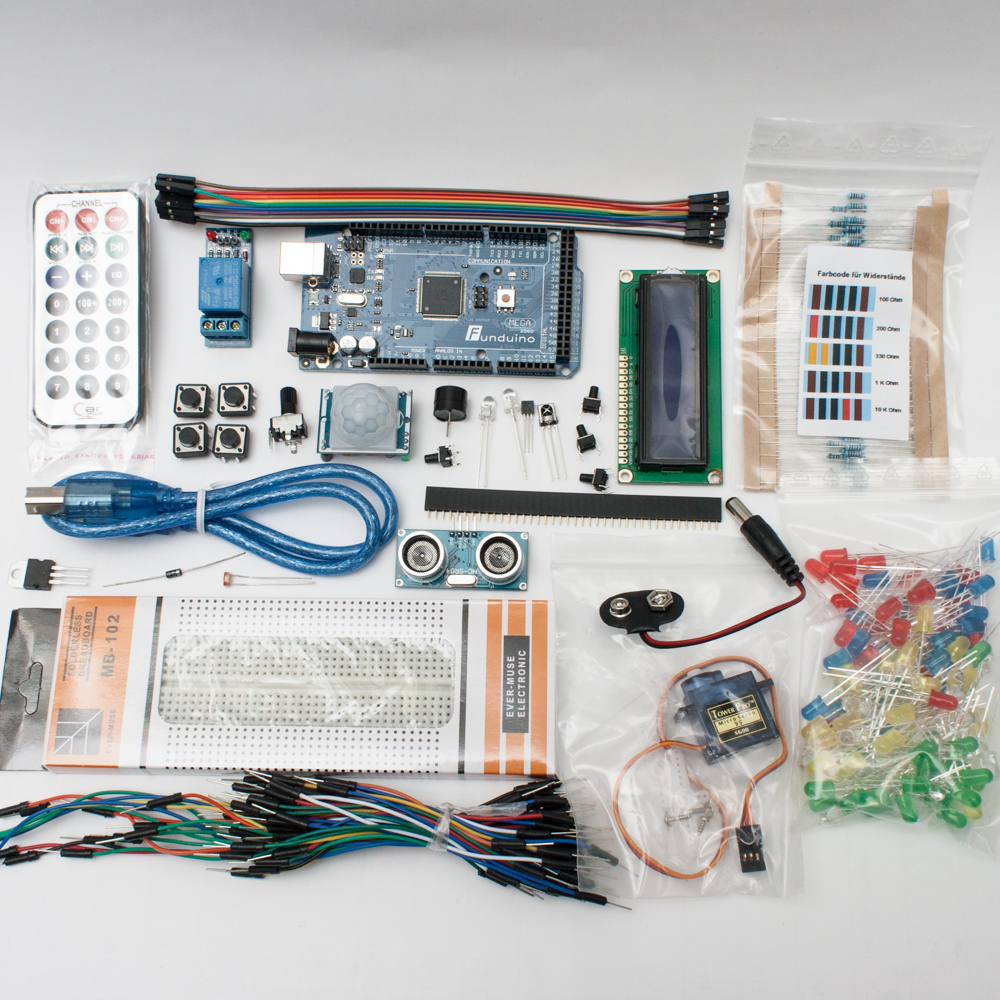
\includegraphics[width=.3\textwidth]{Funduino Lernset 6.jpg}
\includegraphics[width=.3\textwidth]{FunduinoSet6}

\subsection{Funduino-Lernset 1} 
\infobox{1}{5}{Neu}
Nachbau eines Arduinos mit vielen Teilen zum basteln und ausprobieren.\\
\textbf{Teile:} Funduino UNO R3, Sensoren, Bauteile (details siehe QR-Code)
% http://funduino.de/index.php/shop/lernsets/produkt1alias

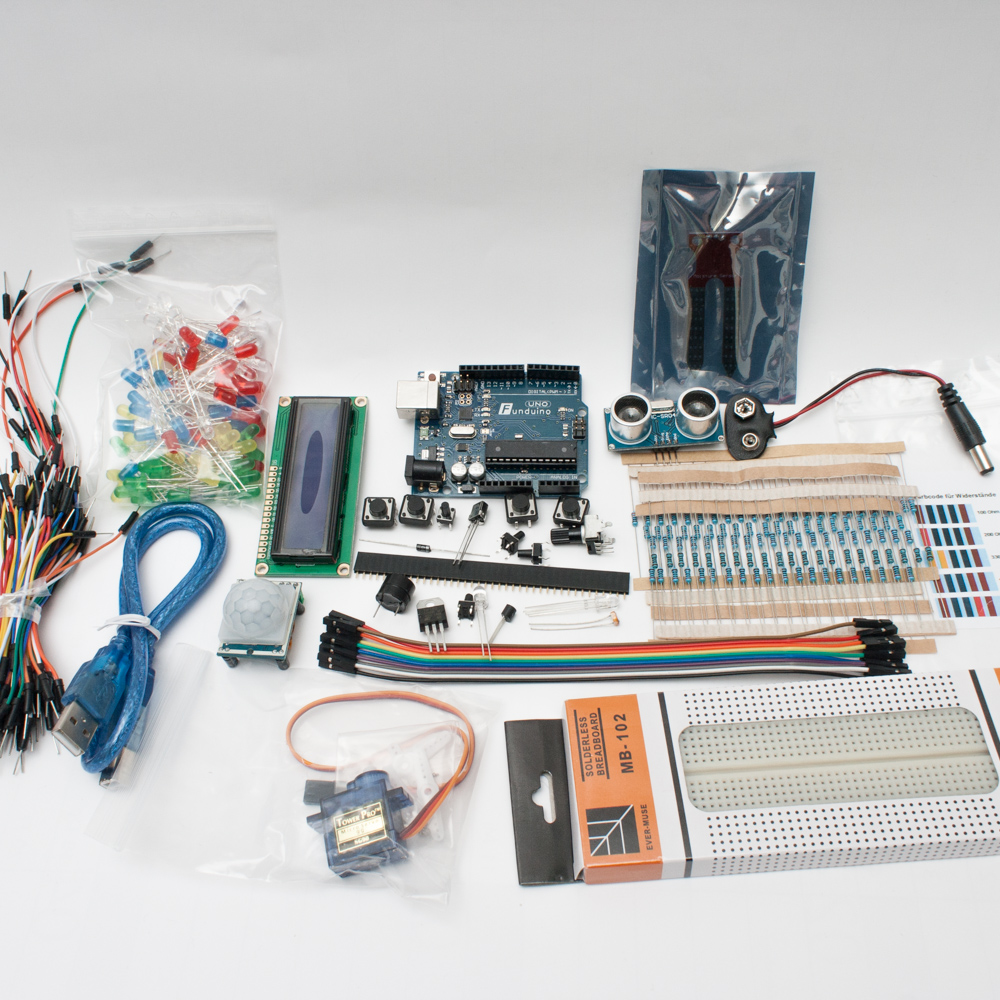
\includegraphics[width=.3\textwidth]{Funduino Lernset 1.jpg}
\includegraphics[width=.3\textwidth]{FunduinoSet6}

\subsection{Odroid XU3} 
\infobox{1}{0}{Neu}
Profi Variante eines Miniatur-Computers der unteranderem einen Quadcore hat.\\
\textbf{Teile:} Odroid XU3, Netzteil 4A, Gehäuse, 16GB eMMC 5.0 XU3 Linux, 16GB eMMC 5.0 XU3 Android

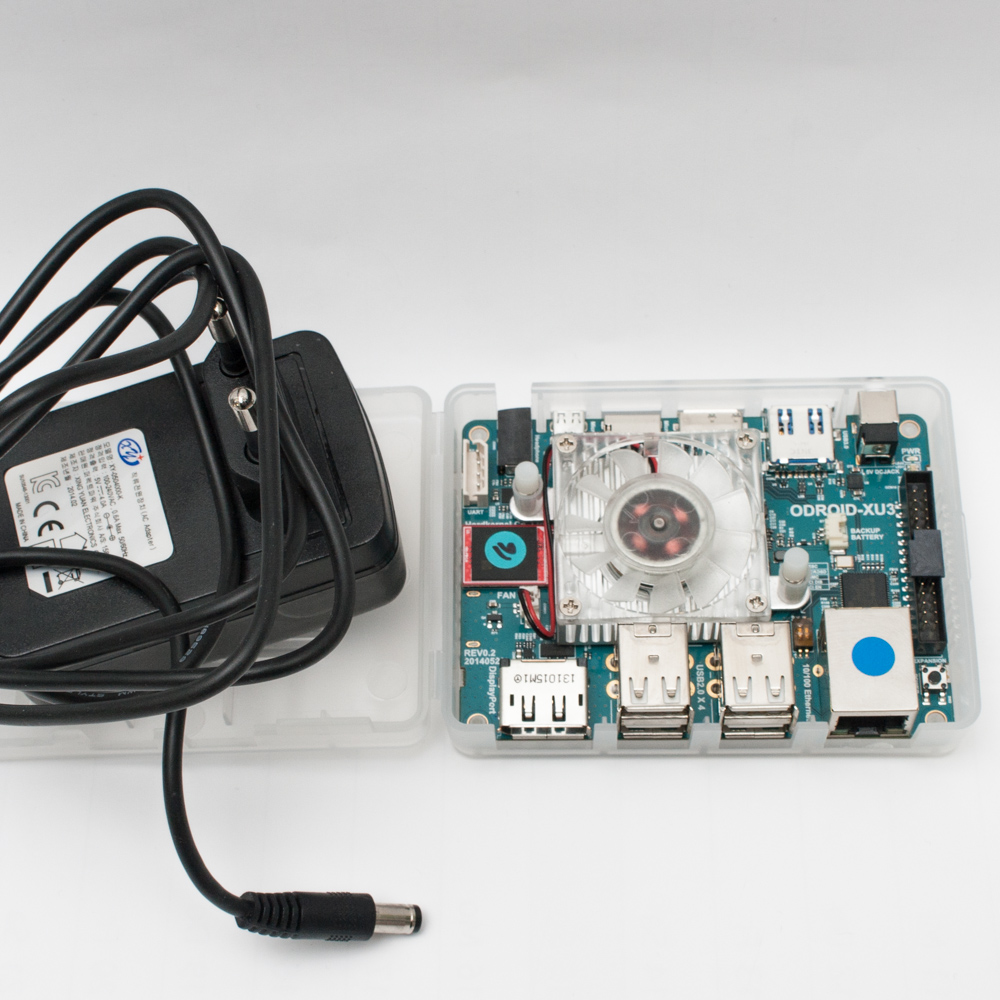
\includegraphics[width=.3\textwidth]{Odroid XU3-2.jpg}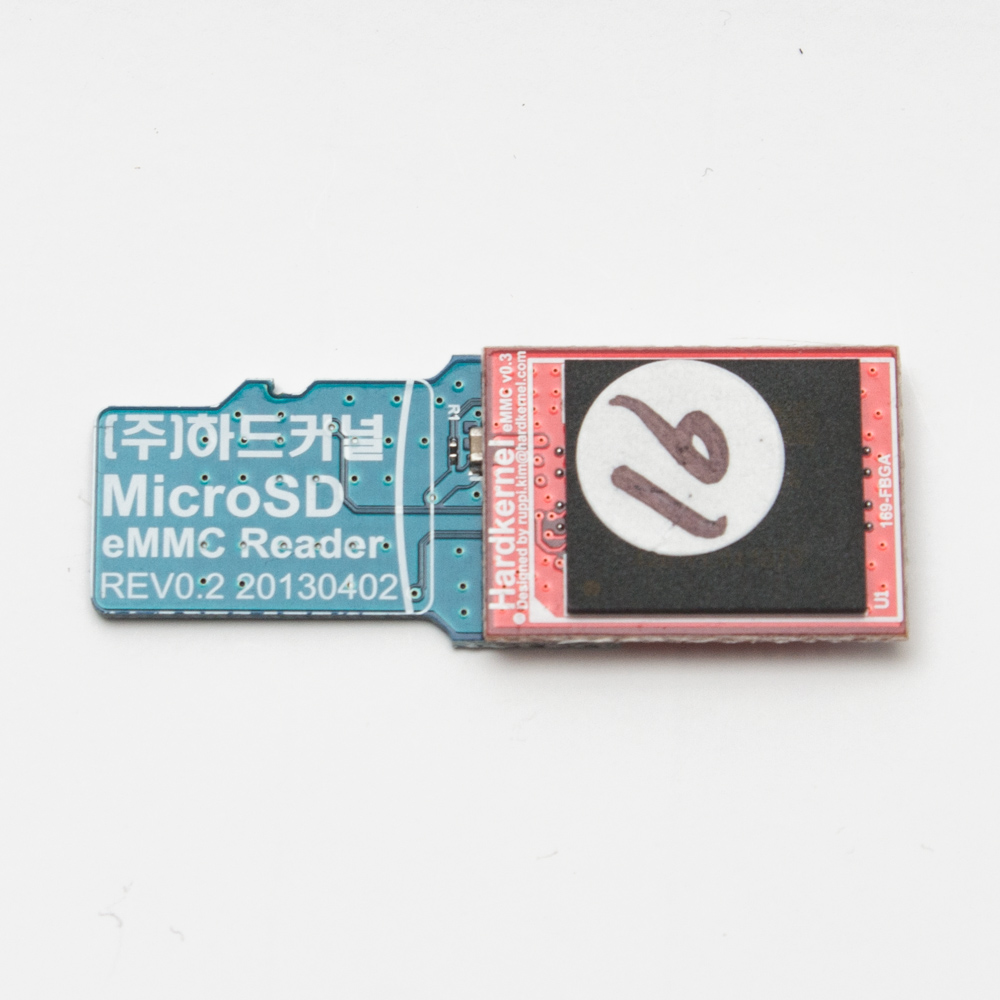
\includegraphics[width=.3\textwidth]{eMMC 16GB.jpg}
\includegraphics[width=.3\textwidth]{Odroid}

\subsection{Kartenlesegerät}
\infobox{2}{0}{Neu}
Einfaches Kartenlesegerät für verschiedene SD-Karten.\\
\textbf{Teile:} Multikartenlesegerät (SD-Karten etc.)

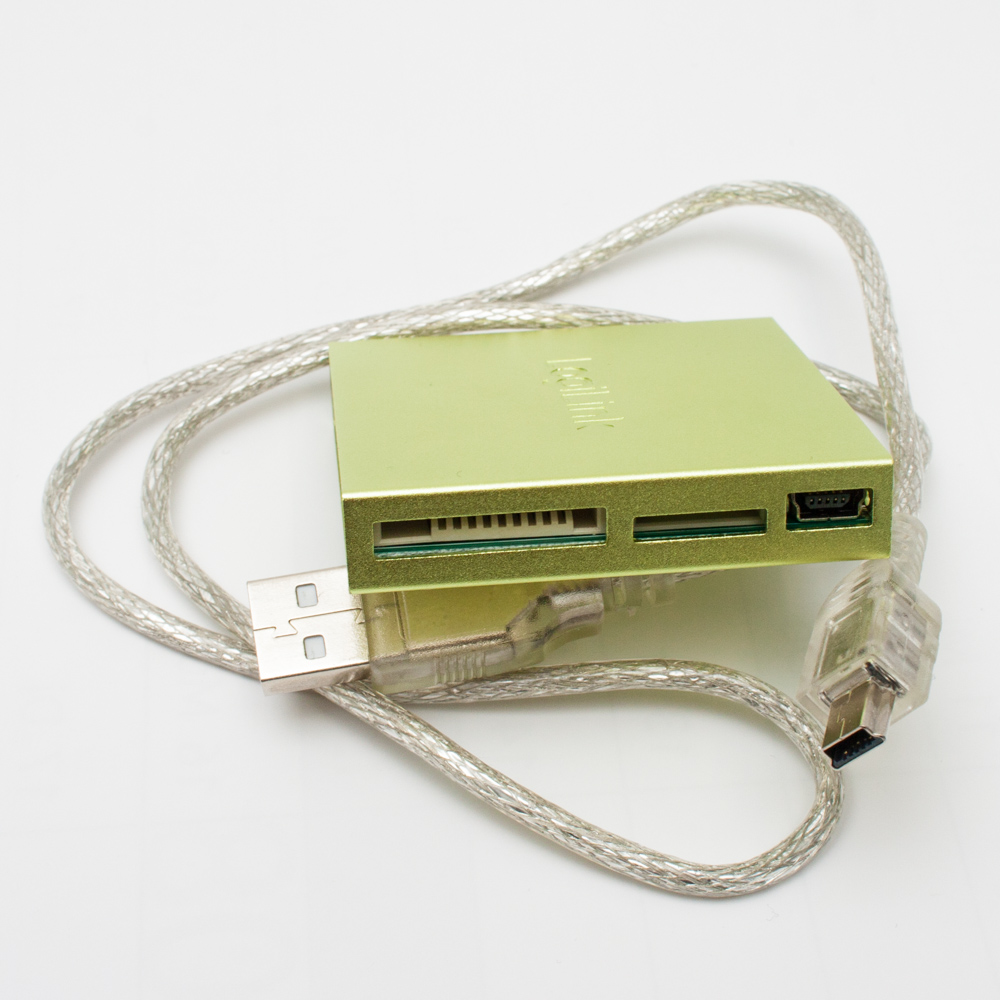
\includegraphics[width=.3\textwidth]{Kartenleser.jpg}

\subsection{BrickPi}
\infobox{2}{0}{Neu}
Eine Platine die es ermöglicht an einen Raspberry Pi die Motoren und Sensoren der Lego Mindstorm Serie anzuschließen.\\
\textbf{Teile:} BrickPi Advanced Power

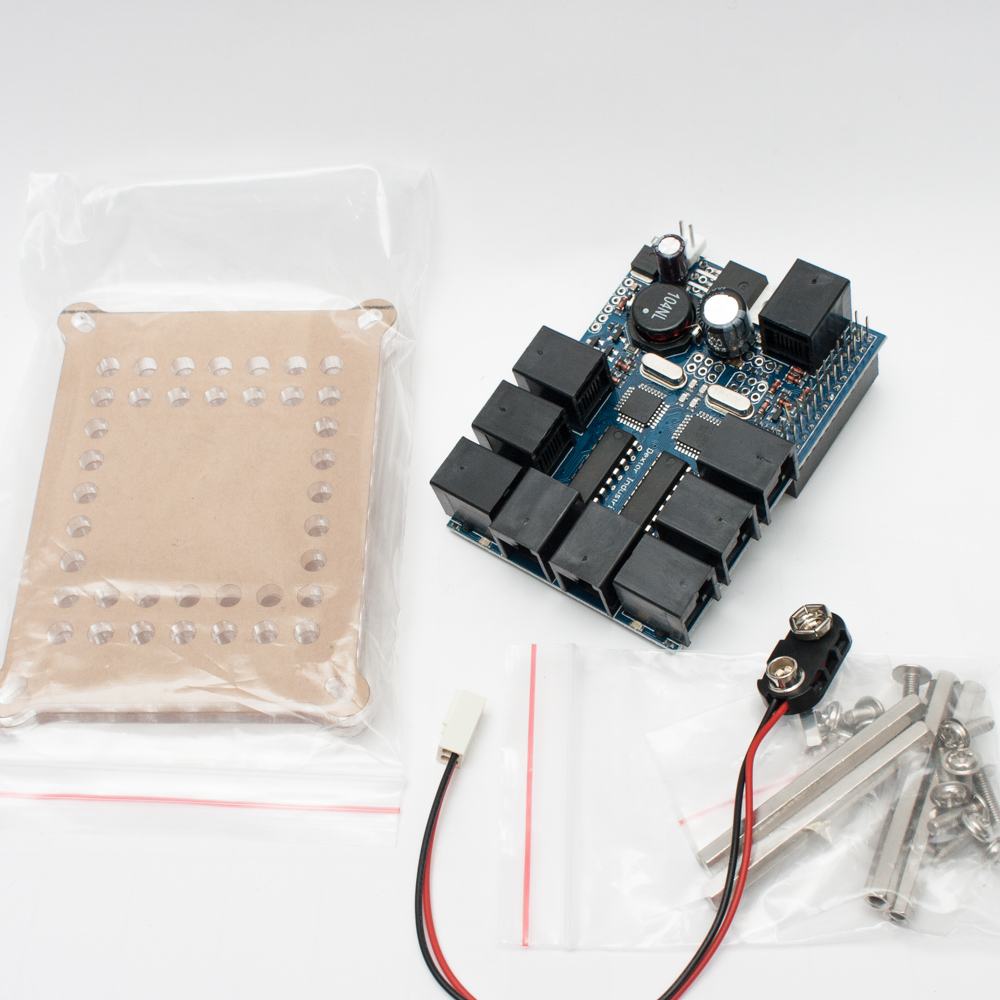
\includegraphics[width=.3\textwidth]{BrickPi.jpg}
\includegraphics[width=.3\textwidth]{BrickiPi}

\subsection{HD Webcam}
\infobox{2}{1,5}{Neu}
Eine HD Webcam. \\ 
\textbf{Teile:} Logitech c920 Webcam

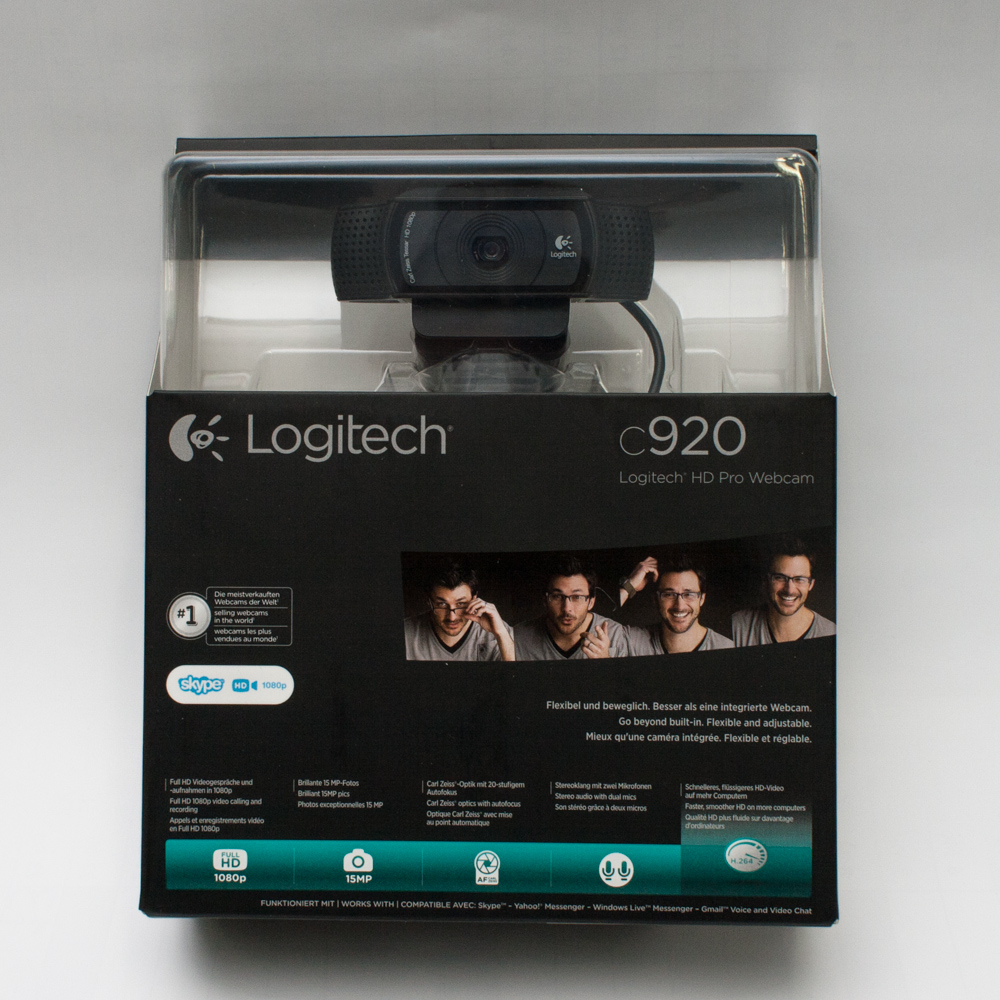
\includegraphics[width=.3\textwidth]{Webcam Logitech C920.jpg}

\section{LEGO}

\subsection{Lego Mindstorms Education Basis Set (EV3)}
\infobox{3}{0}{Neu}
Ein Basis Lego Mindstorms Set mit allen nötigen Teilen um kleine Roboter zu bauen und zu programmieren. Lego 45544. \\
\textbf{Teile:}Ladegerät, NXT-Brick, verschiedene Teile (siehe Auflagebild)

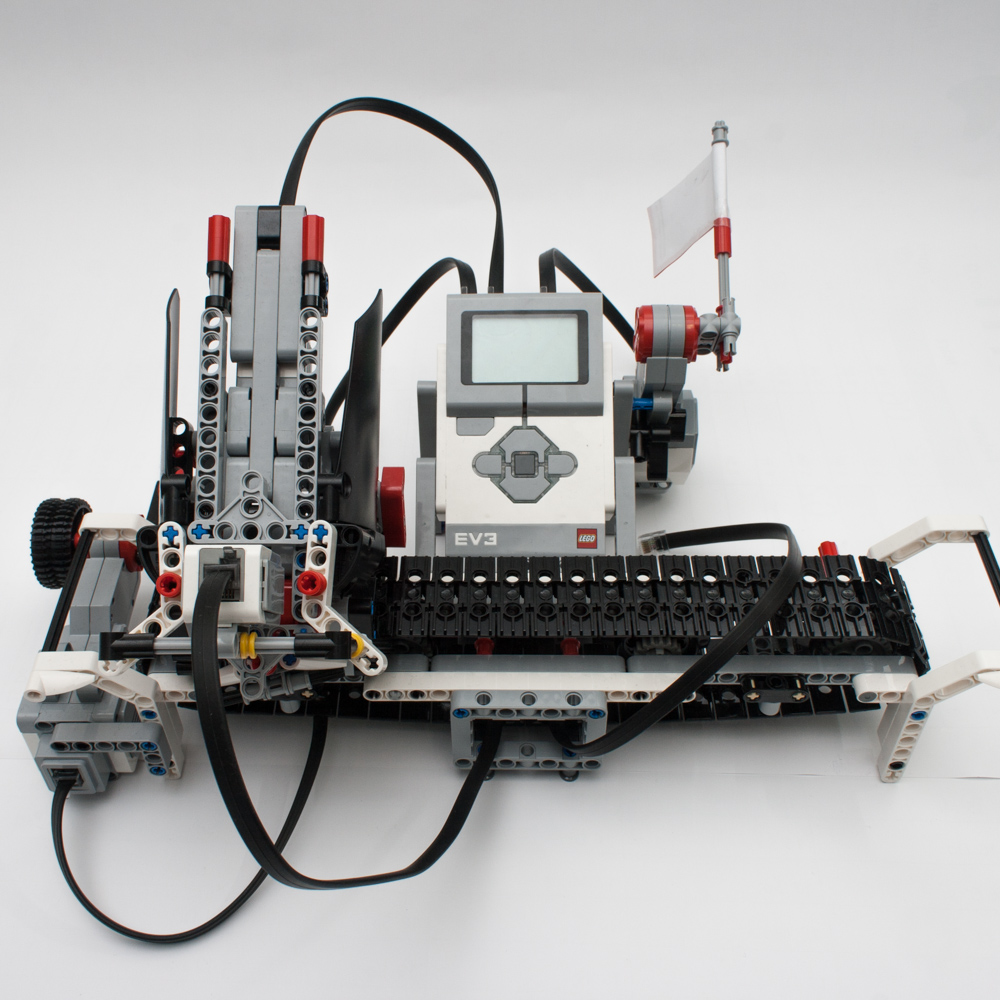
\includegraphics[width=.3\textwidth]{Mindstorms EV3 Edu Core.jpg}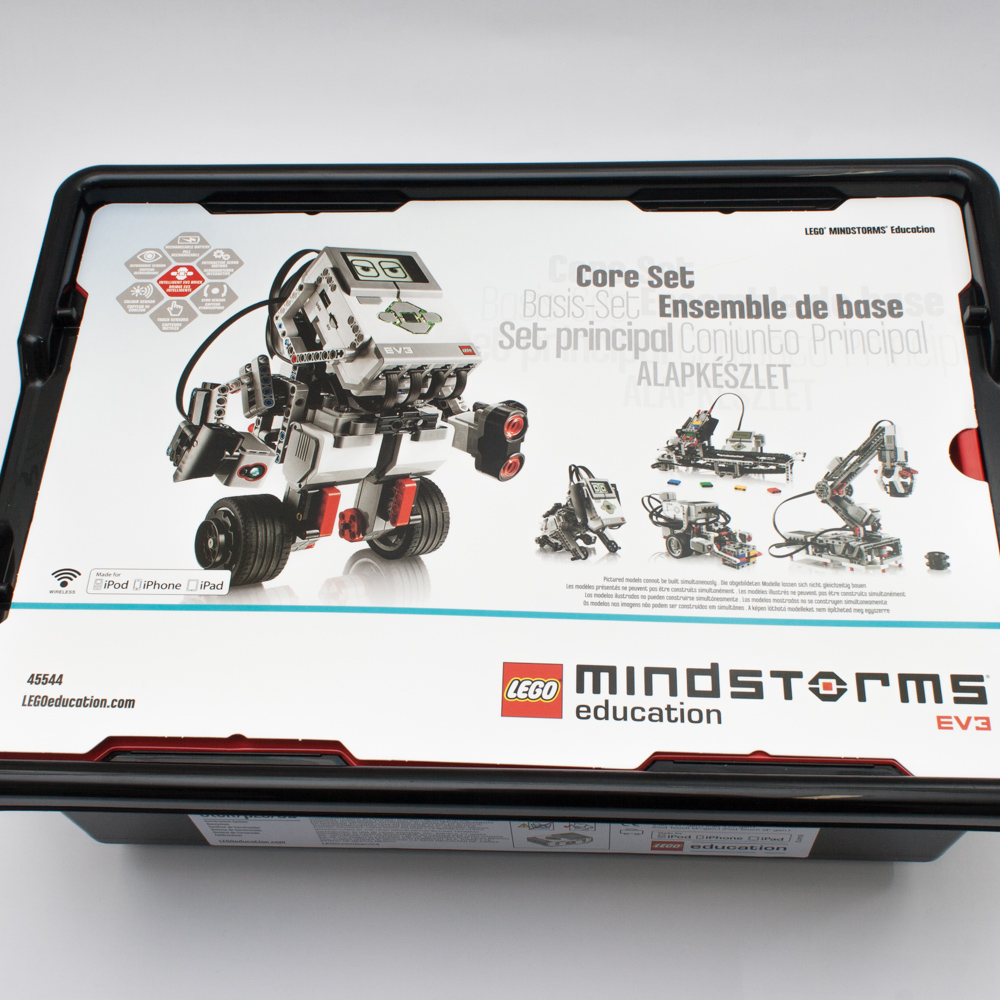
\includegraphics[width=.3\textwidth]{Mindstorms EV3 Edu Core-2.jpg}

%\subsection{Lego Mindstorms Education Expansion Set (EV3)}
%\infobox{3}{0}{Neu}
%Ein Lego-Mindstorms Ergänzungsset mit allen nötigen Teilen. Lego 45560. \\
%\textbf{Teile:} verschiedene Teile

%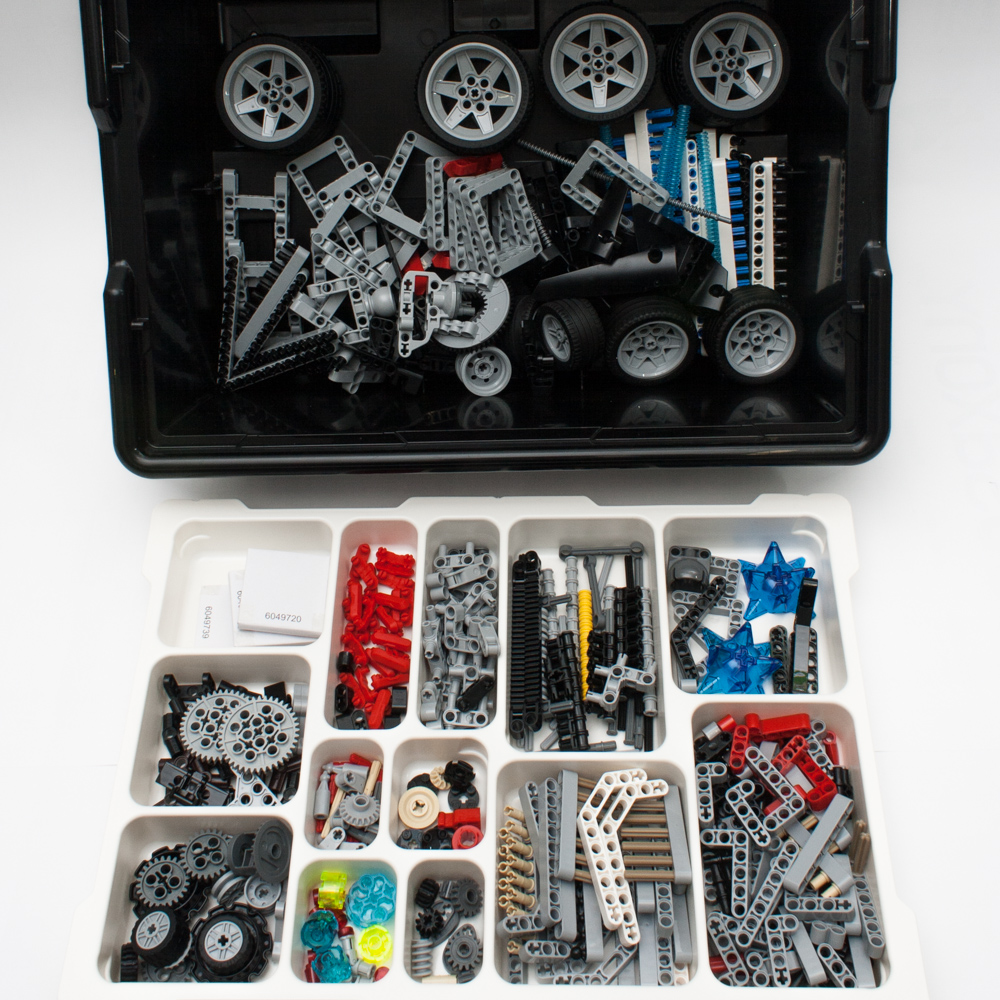
\includegraphics[width=.3\textwidth]{Mindstorms EV3 Edu Expansion.jpg}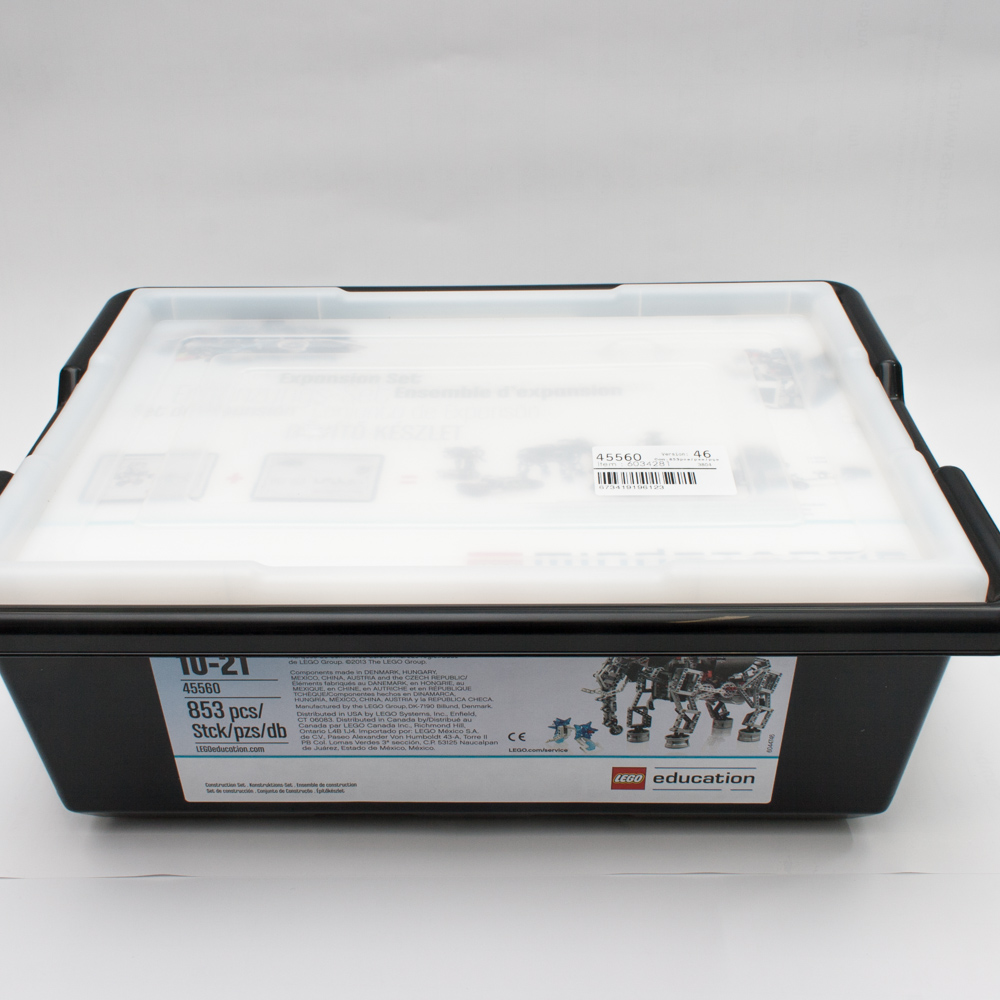
\includegraphics[width=.3\textwidth]{Mindstorms EV3 Edu Expansion-2.jpg}

%\subsection{Lego Mindstorms Set (EV3)}
%\infobox{3}{0}{Neu}
%Ein Basis Lego Mindstorms Set mit allen nötigen Teilen um kleine Roboter zu bauen und zu programmieren. Lego 31313. \\
%\textbf{Teile:} .....

%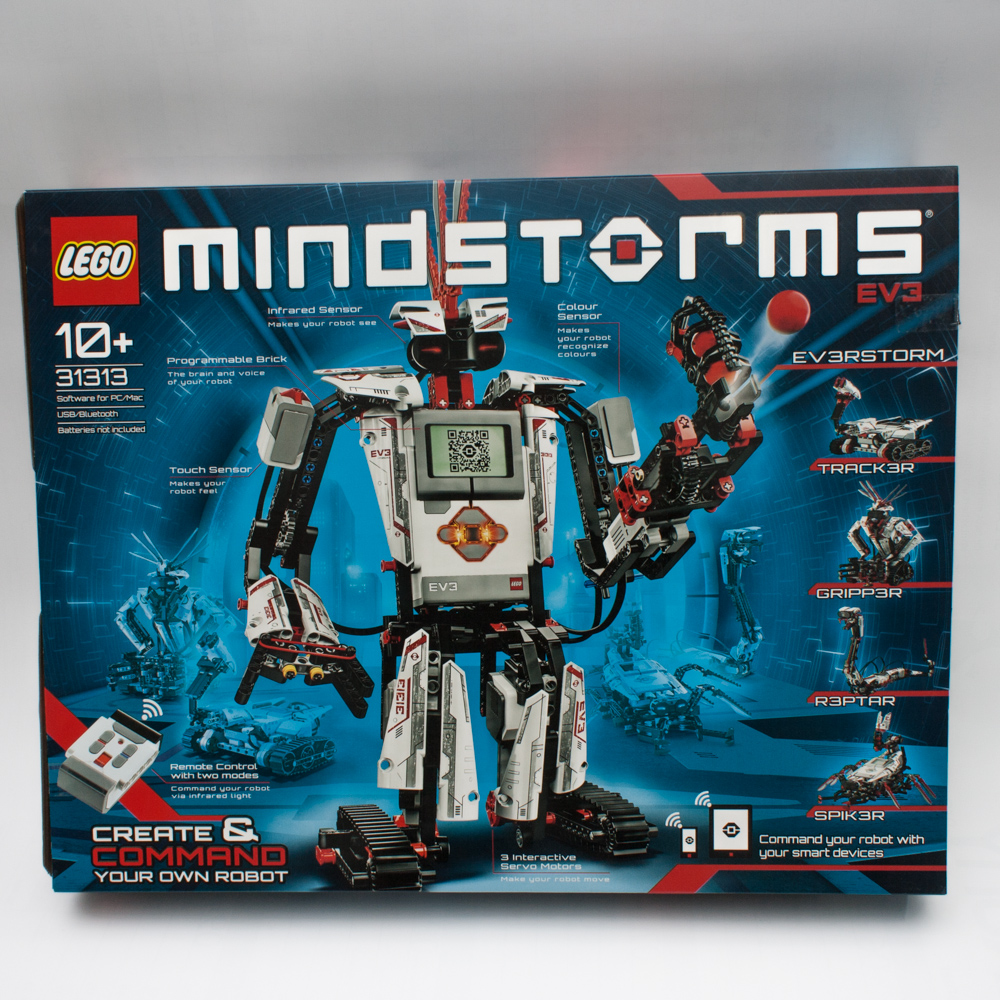
\includegraphics[width=.3\textwidth]{Mindstorms EV3.jpg}

%\subsection{Große Lego Box}
%\infobox{Noch keine}{0}

%
\includegraphics[width=.3\textwidth]{fsrlogo}
\includegraphics[width=.3\textwidth]{fsrlogo}


\section{Gesellschaftsspiele}

\subsection{Nobody is perfect}
\infobox{1}{0}{Neu}
Gesellschaftsspiel für 3-10 Personen. Ravensburger 27225. \\
\textbf{Teile:} Spielplan, Anleitung, Fragekarten Stapel, verschiedene farbige Figuren, Box

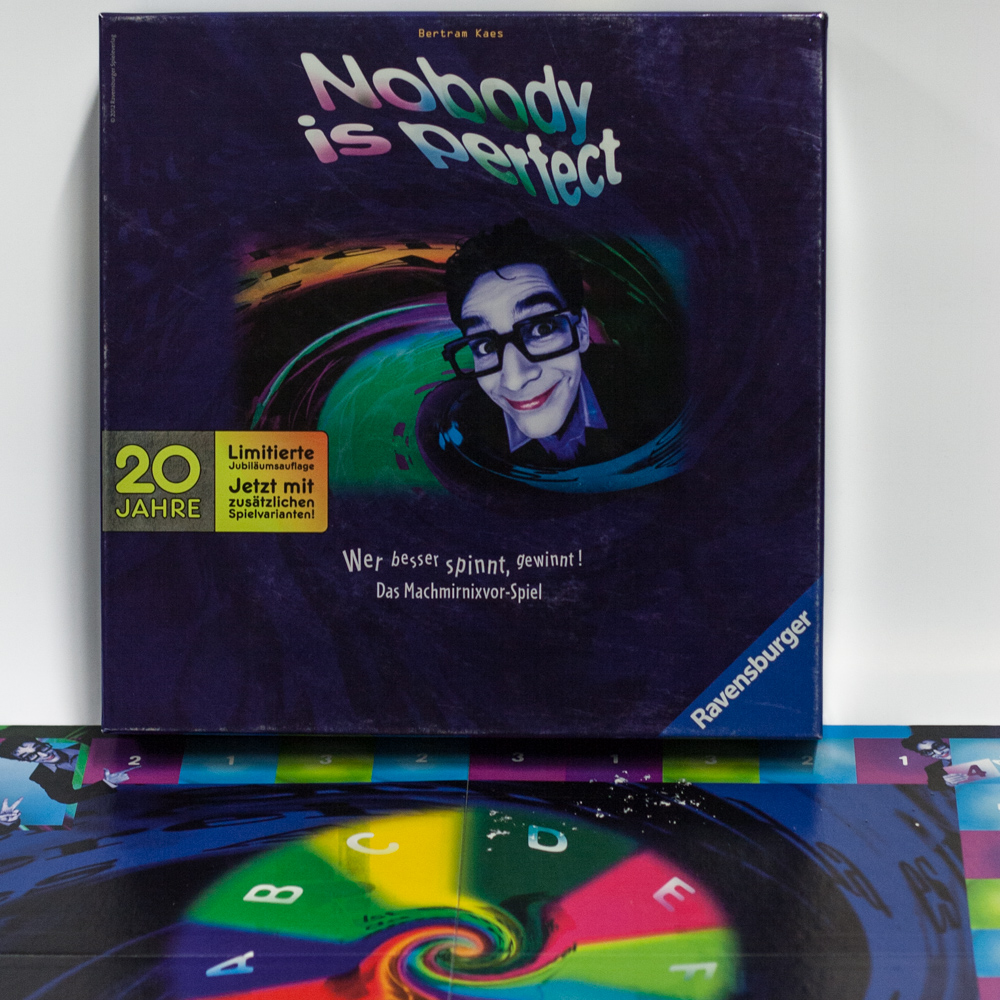
\includegraphics[width=.3\textwidth]{Nobody is perfect.jpg}

%\subsection{Es geht seinen Gang}
%\infobox{1}{0}

\section{Sonstiges}

\subsection{Großer Grill}
\infobox{1}{10}{Neu}
Ein Edelstahl Barbecue Holzkohlegrill mit einer Grillfläche von 600 cm$^2$. \\
\textbf{Teile:} Rost, Grill
%
\includegraphics[width=.3\textwidth]{fsrlogo}
\includegraphics[width=.3\textwidth]{fsrlogo}
\includegraphics[width=.3\textwidth]{fsrlogo}

%\subsection{Marc}
%\infobox{1}{Over 9000}
%Sie suchen Ordnung und Struktur im Leben? Leihen sie jetzt einen Marc und ihre Träume werden wahr! Er kommt in einer handlichen $2m \times 0,5m$  Box, rufen sie jetzt an und sie erhalten einen {\em Labeldrucker} gratis dazu! \\
%
\includegraphics[width=.3\textwidth]{fsrlogo}


\end{document}
